\documentclass{article}

% Language setting
% Replace `english' with e.g. `spanish' to change the document language
\usepackage{biblatex} %Imports biblatex package
\addbibresource{refs.bib}
\usepackage[english]{babel}
\usepackage{array}
\usepackage{amsmath}
\usepackage{pythonhighlight}
\usepackage{multirow}
\newcolumntype{P}[1]{>{\centering\arraybackslash}p{#1}}
\newcolumntype{M}[1]{>{\centering\arraybackslash}m{#1}}

% Set page size and margins
% Replace `letterpaper' with `a4paper' for UK/EU standard size
\usepackage[letterpaper,top=2cm,bottom=2cm,left=3cm,right=3cm,marginparwidth=1.75cm]{geometry}

\usepackage{amsmath}
\usepackage{graphicx}
\usepackage[colorlinks=true, allcolors=blue]{hyperref}
\usepackage{setspace}
\usepackage{booktabs}
\usepackage[T1]{fontenc}
\usepackage{longtable}
\doublespacing

\begin{document}
\begin{titlepage}

\centering
\scshape
\vspace{\baselineskip}

%
\rule{\textwidth}{1.6pt}\vspace*{-\baselineskip}\vspace*{2pt}
\rule{\textwidth}{0.4pt}

{\Huge \textbf{\textsc{ Tensile Stress-Strain \\
\vspace{15pt}}}}

\rule{\textwidth}{0.4pt}\vspace*{-\baselineskip}\vspace{3.2pt}
\rule{\textwidth}{1.6pt}\vspace{6pt}
\centerline{\textit{University of Illinois at Urbana-Champaign}} 
\centerline{\textit{Department of Nuclear, Plasma, and Radiological Engineering}}
\vspace{1.5\baselineskip}


\large \centerline{\textbf{Author:} Nathan Glaser}
\large \centerline{\textbf{Net-ID:} nglaser3}
\quad

\vfill
\large \centerline{September 25, 2024}
%
\pagenumbering{gobble}
\end{titlepage}

\tableofcontents
\newpage
\pagenumbering{arabic}

\section{Abstract}
Hardness, strength, and ductility of materials are all exceedingly important quantities to have an understanding of prior to the usage or deployment of engineering materials. One of the most common ways to test for these values is through a uniaxially loaded stress state, called a tension test. We conducted tension tests on 8 materials to determine these quantities. We investigated Aluminum Alloy 2024, PMMA, Cold Rolled 1018 Steel, 304 Stainless Steel, 1045 Steel (both Cold Rolled and Annealed), Aluminum Alloy 7075, and Bronze. We determined the elastic moduli, yield strengths, ultimate tensile strengths, percent of elongation, modulus of resilience, and hardness values on the Rockwell B scale. We investigated the change of these values as a function of material hardness. Further, we investigated the differences between true and engineering stress/strain, and the applicability of a power-law fit to the plastic deformation region of the true stress/strain curve of 304 Stainless Steel. Lastly, we investigated the effects of plastic deformation on the elastic modulus and yield strength of Bronze. We found that material properties pertaining to strength, elasticity, and ductility vary strongly with hardness. We found true stress is larger than engineering, and true strain is smaller than engineering, and that a power-law fit is well adept to approximating the plastic deformation region of the stress/strain curve for 304 Stainless Steel. Finally, we found that as plastic deformation increases so does the yield strength of the material, conversely the elastic modulus decreases slightly. 
\newpage
\section{Introduction}
An exceedingly common loading condition to test for engineering materials strength and deformation properties is uniaxially. An example of this type of loading condition is a tension or compression test, in which the specimen is loaded and either pulled / compressed until failure or the desired outcome fruitions. These tests measure the stress, the axial force applied to the specimen, and the strain, the dimensional change the specimen undergoes due to loading.
\subsection{Stress and Strain}
Tension and compression tests both load and measure axially, and thus do not take into consideration non-1D changes in geometry. Thus, these tests yield what is commonly named 'engineering' stress/strain. To determine the engineering stress/strain is very simple. The strain is simply how much the specimen is compressed due to the load and is directly measured by the testing apparatus. The stress is simply the force applied by the testing apparatus divided by the cross sectional area of the point of interest on the specimen. 
\begin{equation}
    \sigma_e = \frac{F}{A_o}
    \label{eq:engstress}
\end{equation}

Next, to adjust engineering stress/strain to closer represent the stress and strain the point of interest in the specimen actually undergoes, we utilize Eqs. \ref{eq:trustress} and \ref{eq:trustrain} to convert to true stress/strain.

\begin{equation}
    \sigma_t = \sigma_e \left(1+ \epsilon_e \right)
    \label{eq:trustress}
\end{equation}
\begin{equation}
    \epsilon_t = ln\left(1+\epsilon_e\right)
    \label{eq:trustrain}
\end{equation}

\subsection{Elastic and Plastic Deformation}
Materials undergo two types of macroscopic deformation: Elastic and Plastic. Elastic deformation is characterized as deformation that the material can 'spring' back from, or recover from, and revert to its initial geometry prior to the most recent loading phase. Elastic deformation, as visualized on an engineering stress/strain plot, is the region in which the stress is linearly related to the strain, with the slope of this region being the Young's modulus (elastic modulus or E are common pseudonyms). The general equation for elastic modulus is Eq. \ref{eq:elasmod}. 
\begin{equation}
    \sigma = E\epsilon
    \label{eq:elasmod}
\end{equation}

Plastic deformation is characterized as deformation that the material cannot recover from. In this region, the relationship between stress and strain is more complicated, but is typically approximated using Eq. \ref{eq:powlaw}, the power law model.
\begin{equation}
    \sigma = K \left( \epsilon\right)^n
    \label{eq:powlaw}
\end{equation}

\subsection{Strength and Hardness}
Various metrics are utilized to quantify the strength and hardness of a material. First, to quantify strength a common metric is the 0.2\% Offset Yield Strength (henceforth simplified to Yield Strength) in which a line with slope equalling the elastic modulus and an x-intercept at 0.2\% strain is used. The intersection point of the linear line and the stress-strain curve is the Yield Strength. Further, the Ultimate Tensile Strength (henceforth UTS) is simply the maximum engineering stress the specimen endures. Next, various quantities are utilized to measure a material's hardness. Various tests are utilized: Rockwell A/B/C, Brinnel, Vickers, and more. These utilize an indenter, and forcibly indent a material. The residual indentation is measured and inserted into respective equations to yield hardness values. Another means to quantify a material's hardness is through the modulus of resilience, found utilizing Eq. \ref{eq:modresil}:

\begin{equation}
    U_r = \frac{\left(\sigma_y\right)^2}{2E} 
    \label{eq:modresil}
\end{equation}

where $\sigma_y$ and $E$ are the Yield Strength and Elastic Modulus, respectively. 

\section{Experimental Methods}
To begin, we obtained our various tensile specimens. We gather one tensile specimen for each of the following materials: Aluminum Alloy 2024, PMMA, Cold Rolled 1018 Steel, 304 Stainless Steel, Cold Rolled 1045 Steel, Normalized (Annealed) 1045 Steel, and Aluminum Alloy 7075. For each tensile specimen, except for PMMA and Bronze, we obtained three Rockwell C hardness reading on the grip of the specimen, and recorded the average. Next, we measured the grip and gage diameter of each specimen with a caliper, again three times, and recorded the average. Next, for all specimen, we loaded the specimen into the Instron Load Frame, placed the extensometer on the specimen, and clamped it in. We adjusted the clamps until roughly 90\% of the grip was within the clamp.  We then set the measurement rate to 5mm / min for all materials except PMMA which was set to 1mm / min. We then tested until fracture, except for Bronze in which we cyclically loaded until failure --- relaxed the load applied to the specimen and then revamped the load application two times to have a total of 3 elastic regions. After fracture occurred we measured the fracture diameter three times and recorded the average.
\newpage
\section{Results}

To begin, we measured the axial load and engineering strain of 6 materials: Aluminum Alloy 2024, 1018 Cold-Rolled Steel, 304 Stainless Steel, both 1045 Normalized Steel and 1045 Cold-Rolled Steel, and finally Aluminum Alloy 7075. Utilizing Eq. \ref{eq:engstress}, we obtained Fig. \ref{fig:q1all}, engineering stress vs strain. We also measured the axial load and engineering strain for PMMA, and again utilizing Eq. \ref{eq:engstress} we plotted engineering stress and strain in Fig. \ref{fig:q1pmma}.
\begin{figure}[!h!]
    \centering
    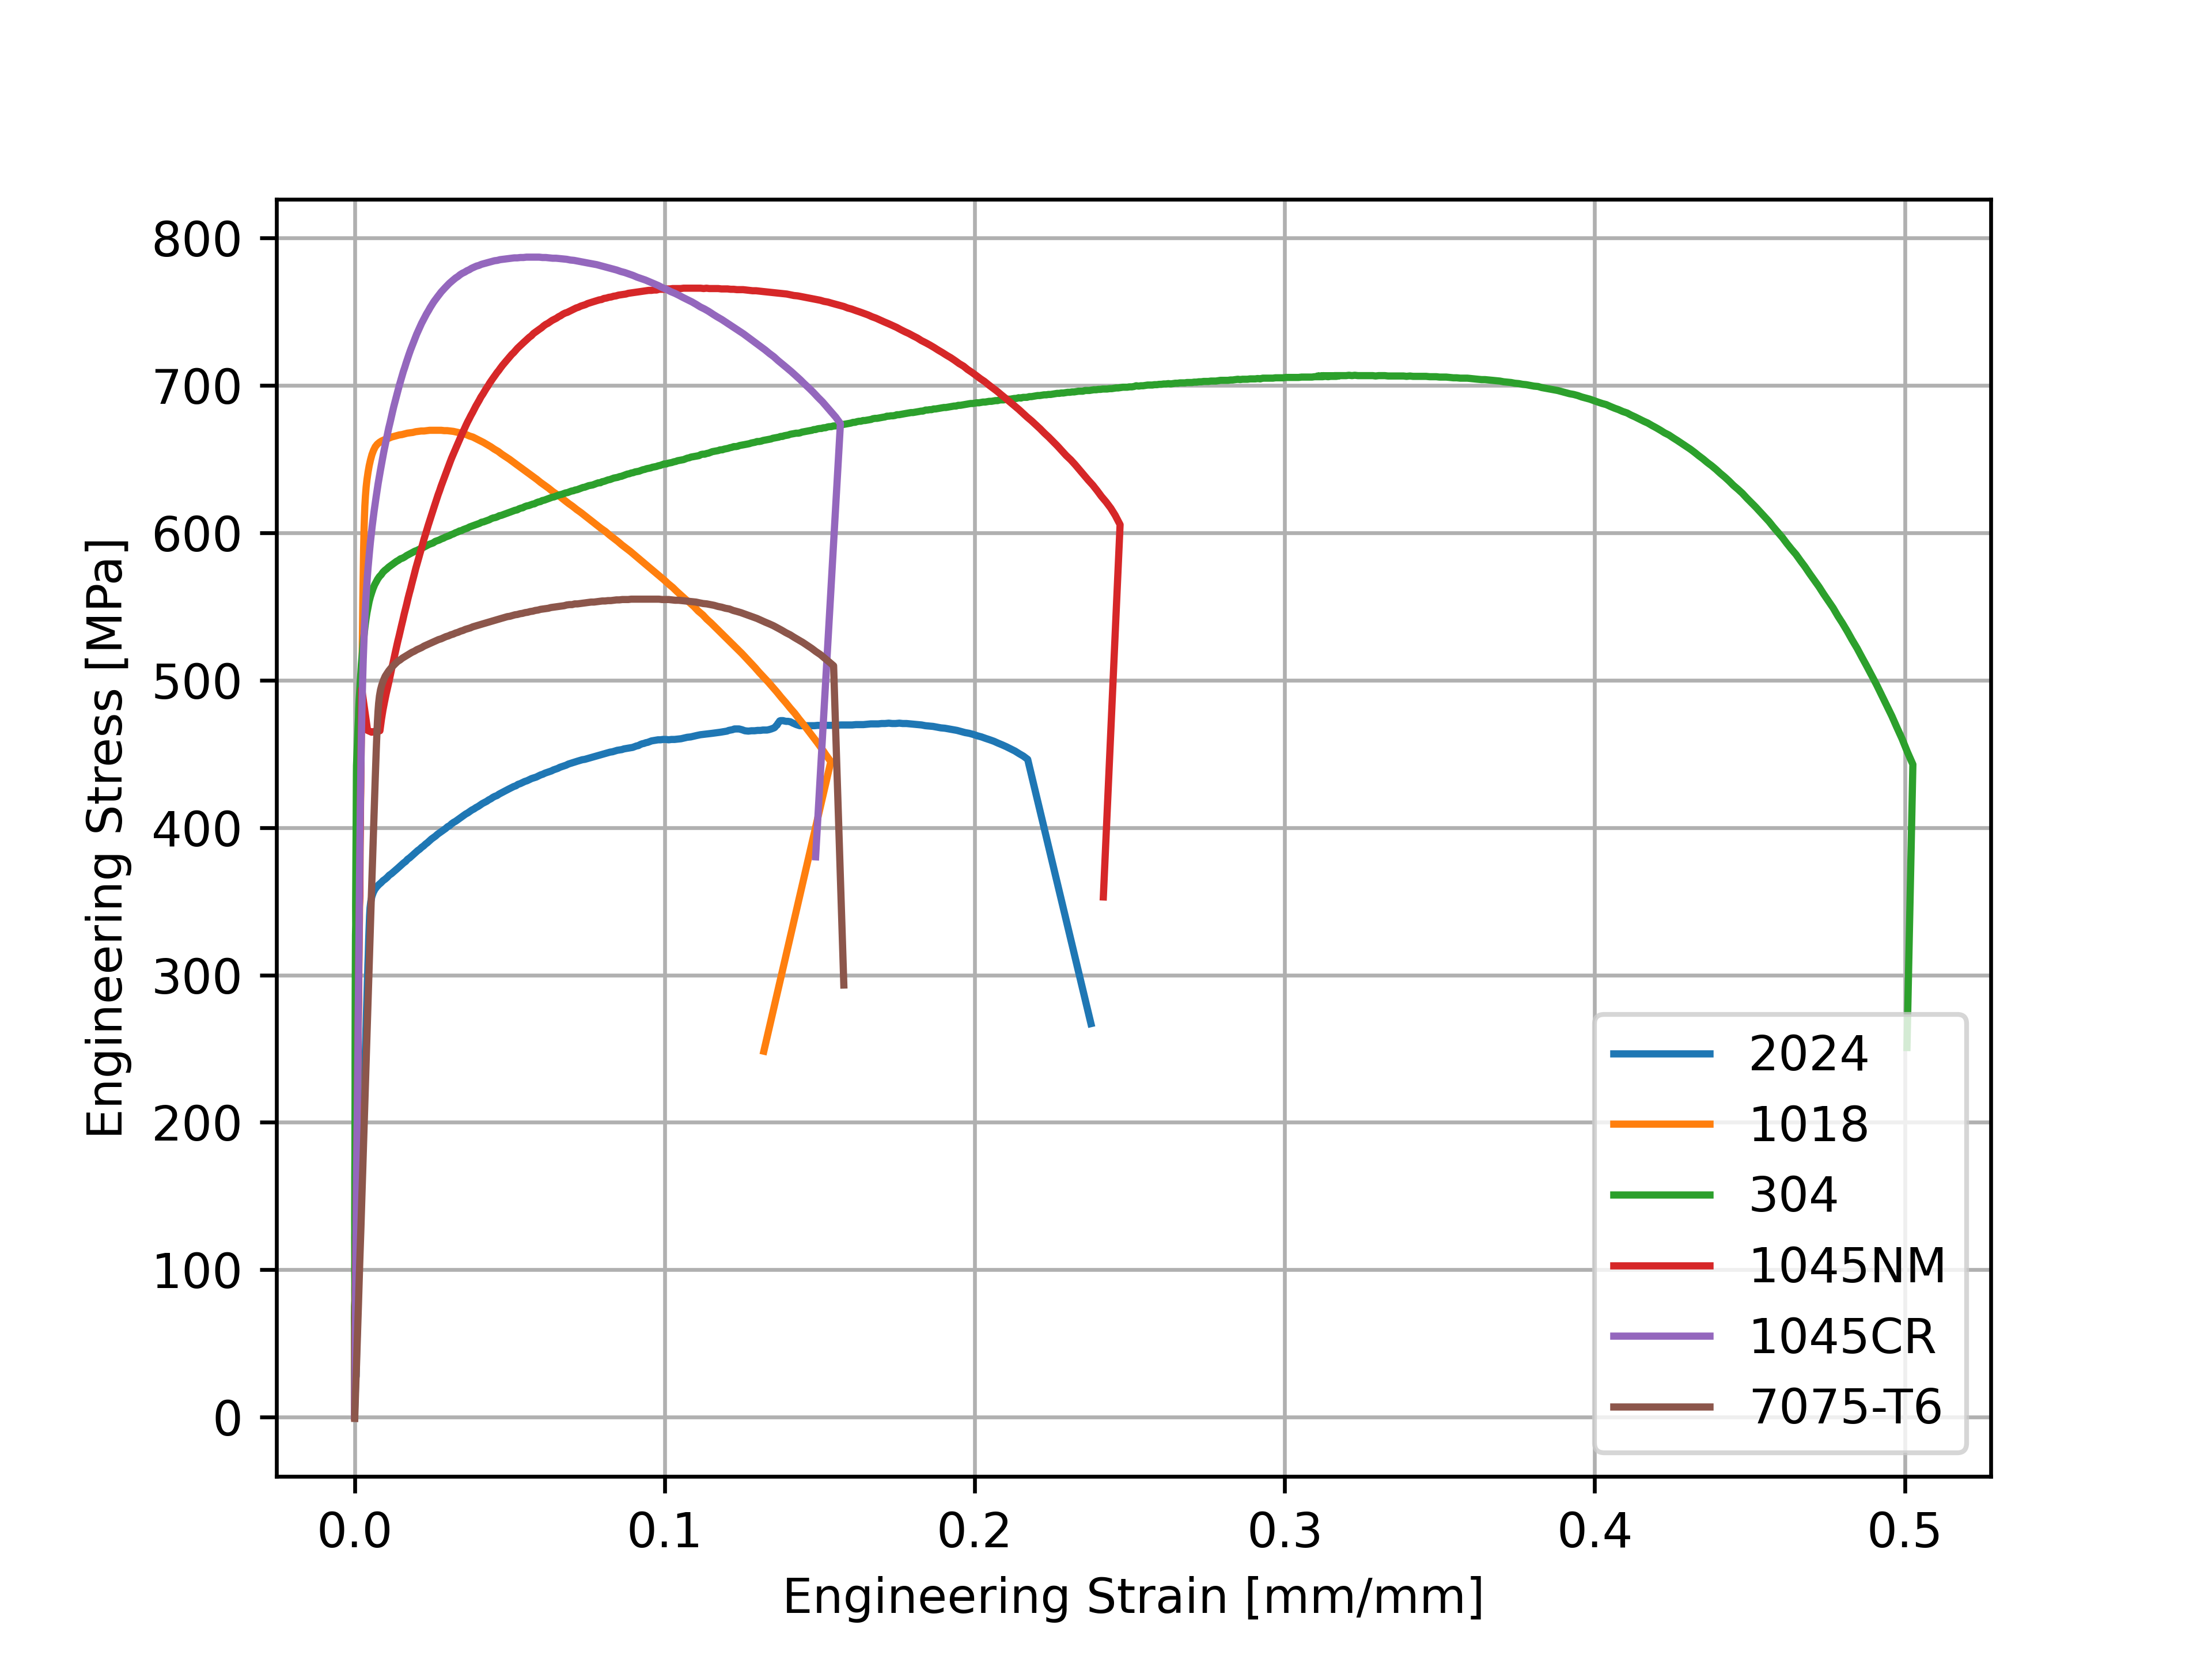
\includegraphics[width=0.6\linewidth]{plots/q1all.png}
    \caption{Engineering stress/strain curve of select materials}
    \label{fig:q1all}
\end{figure}

\begin{figure}[!h!]
    \centering
    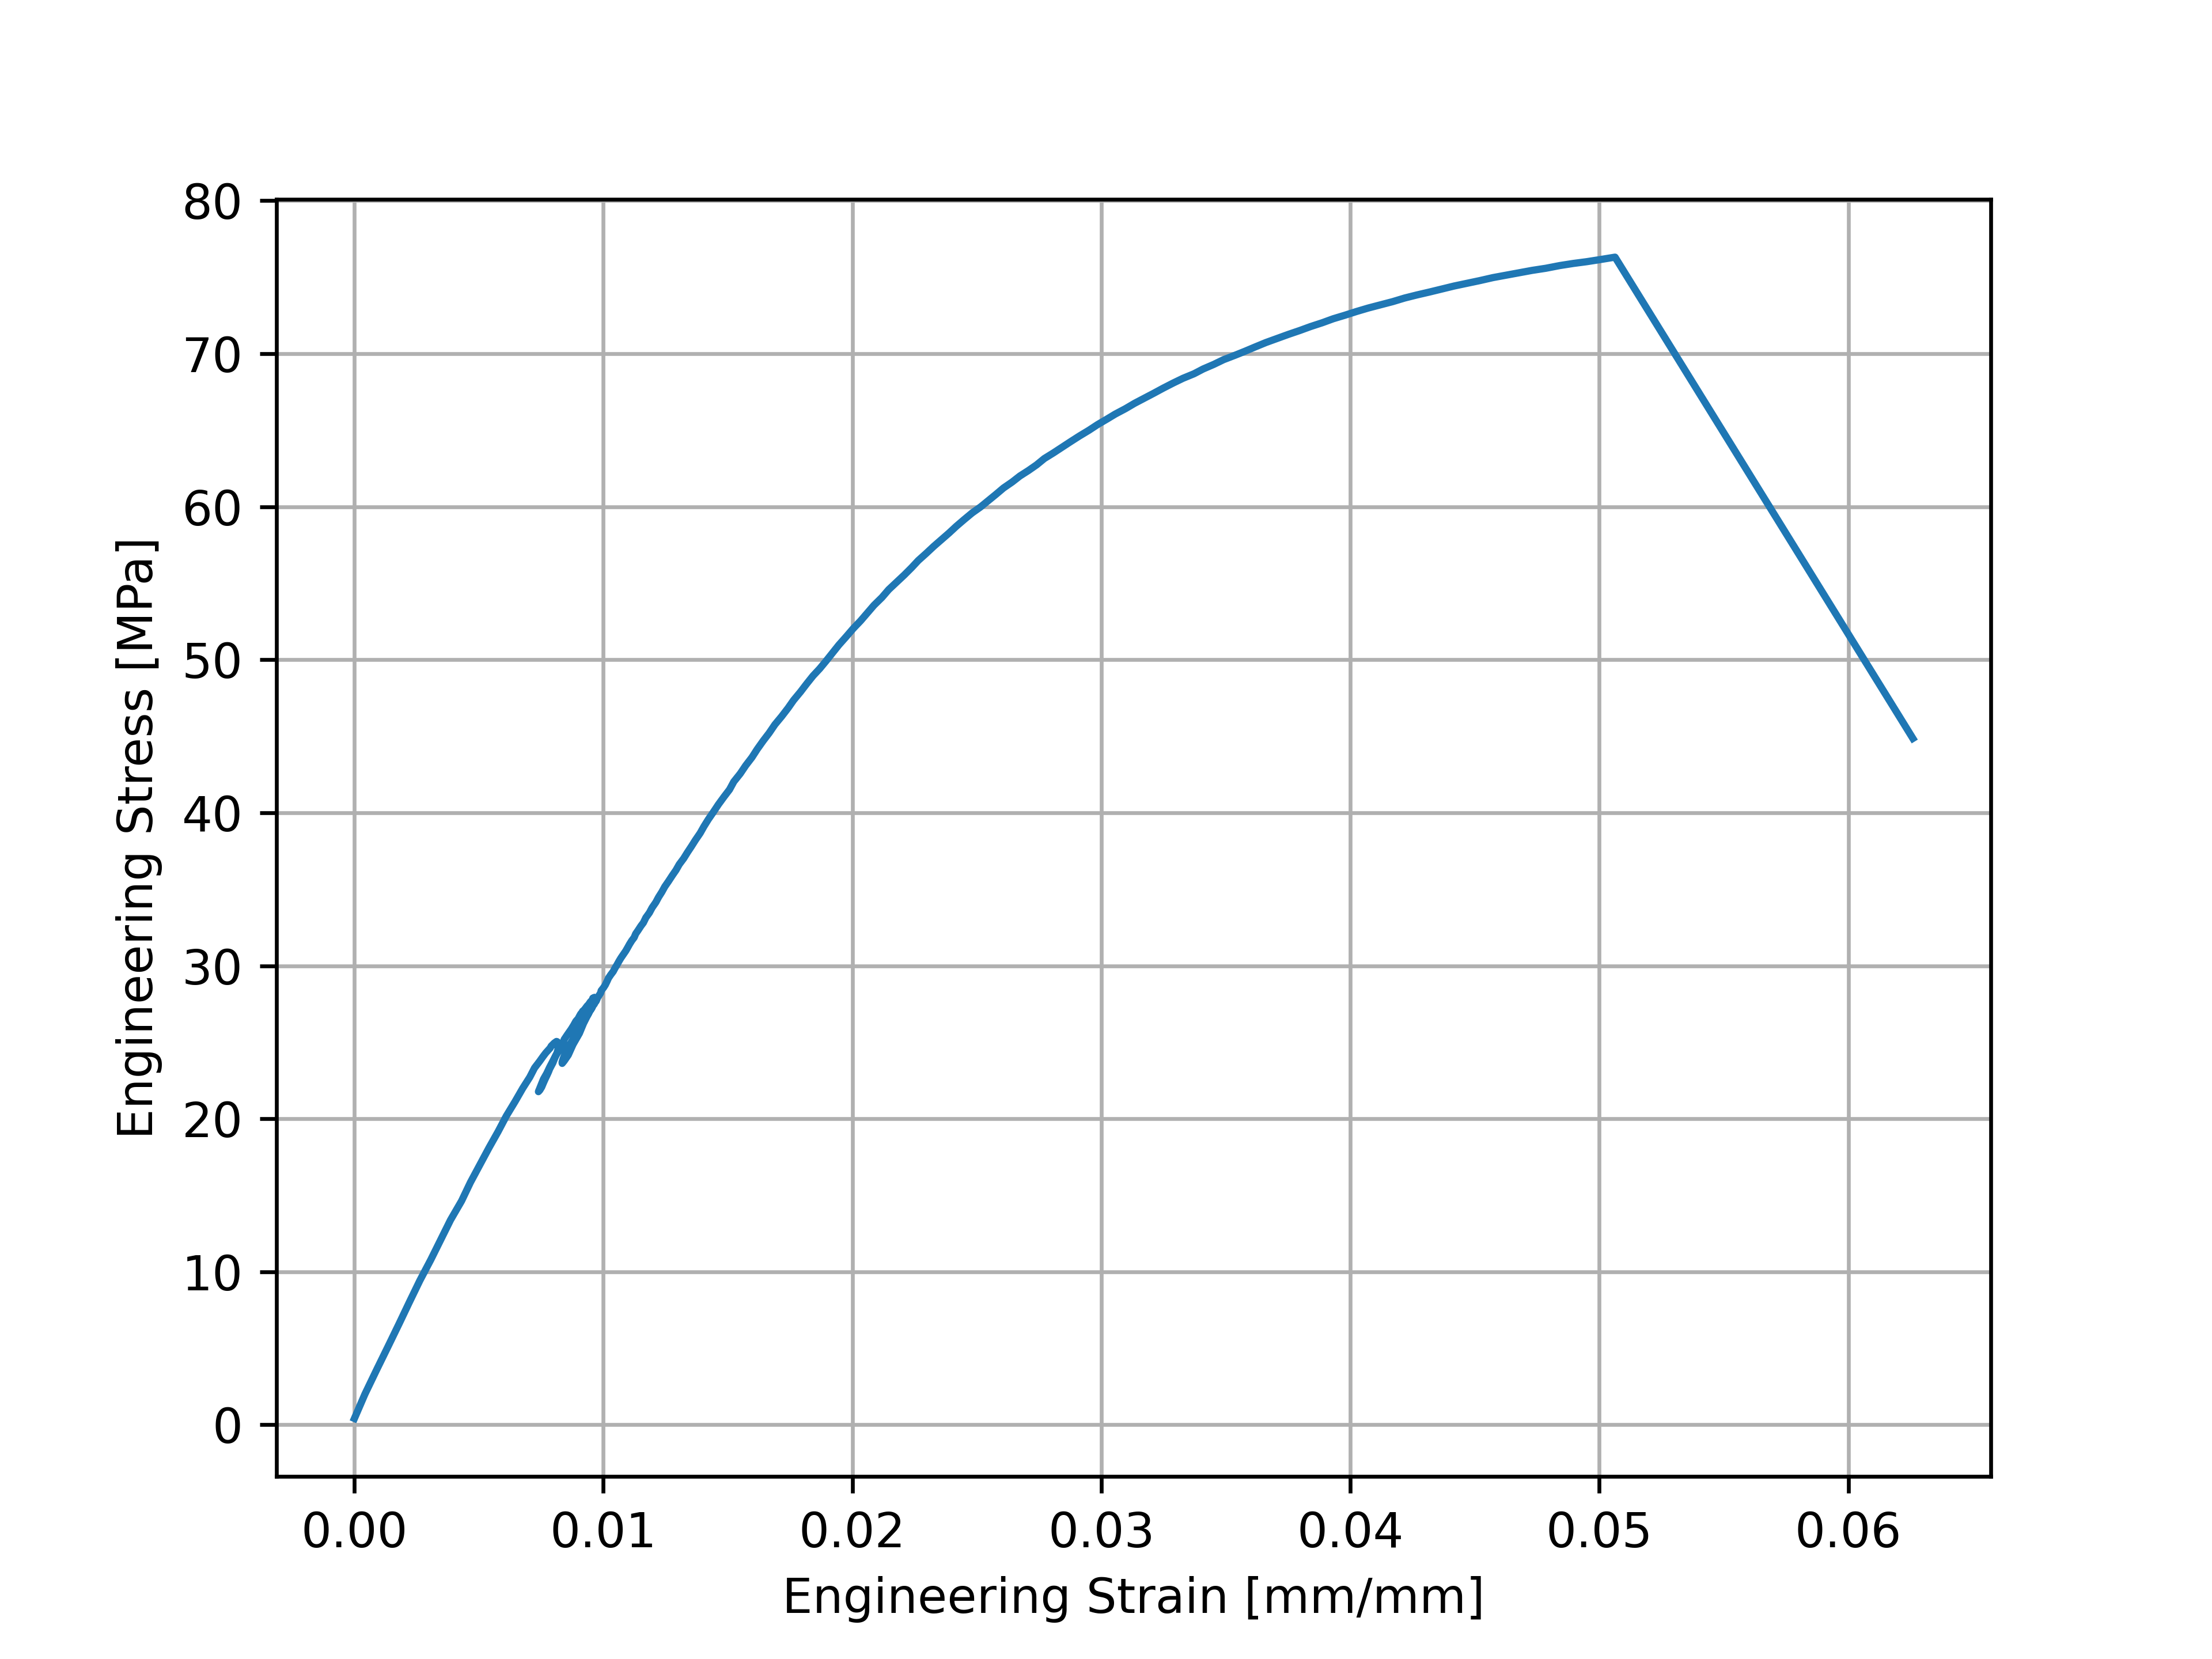
\includegraphics[width=0.6\linewidth]{plots/q1_PMMA.png}
    \caption{Engineering stress/strain curve of PMMA}
    \label{fig:q1pmma}
\end{figure}

\newpage
From the stress-strain curves, and experimentally measured Rockwell-B hardness values (adjusted according to \cite{manual}), we found the Elastic Modulus (Eq. \ref{eq:elasmod}), the Yield Strength (using the 0.2\% Offset method), the UTS, Percent Elongation, and the Modulus of Resilience (Eq. \ref{eq:modresil}). These values are tabulated in Tab. \ref{tab:q2}.
\vspace{.5cm}
\begin{table}[!h!]
    \centering
    \def\arraystretch{1.5}
    \caption{Tensile material properties for selected materials.}
    \begin{tabular}{|c|c|c|c|c|c|c|c|}
         \toprule
         \hline
         \textbf{Material}& \textbf{2024} & \textbf{PMMA} & \textbf{1018CR} & \textbf{304} & \textbf{1045NM} &\textbf{1045CR} & \textbf{7075}\\
         \midrule
         \hline
         \textbf{Elastic Modulus [GPa]}& 71.8 & 3.15 & 204.34 & 670.38 & 203.45 & 220.62 & 66.14 \\
         \textbf{Yield Strength [MPa]} & 359.4 & 42.7 & 649.8 & 525.3 & 465.8 & 583.4 & 501.2 \\
         \textbf{UTS [MPa]} & 472.55 & 76.31 & 669.53 & 706.86 & 765.95 & 787.01 & 554.96 \\
         \textbf{\% Elongated} & 23.75 & 6.26 & 15.36 & 50.26 & 24.69 & 15.67 & 15.77 \\
         \textbf{Mod. of Res.} & 0.9 & 0.29 & 1.03 & 0.21 & 0.53 & 0.77 & 1.9\\
         \textbf{R\textsubscript{B} Hardness} & 72.8 & N/A & 94.3 & 100.6 & 90.7 & 96.1 & 86.8 \\
         \hline
    \end{tabular}
    \label{tab:q2}
\end{table}
\vspace{.5cm}

To continue, we plotted the Elastic Modulus, Yield Strength, the UTS, the Percent Elongation, and Modulus of Resilience as a function of respective material hardness. The resulting Figures are presented in Figs. \ref{figq3:elasmod} - \ref{fig:q3resimod} on the succeeding page. 
\newpage
\begin{figure}[!h!] 
  \begin{minipage}[b]{0.5\linewidth}
    \centering
    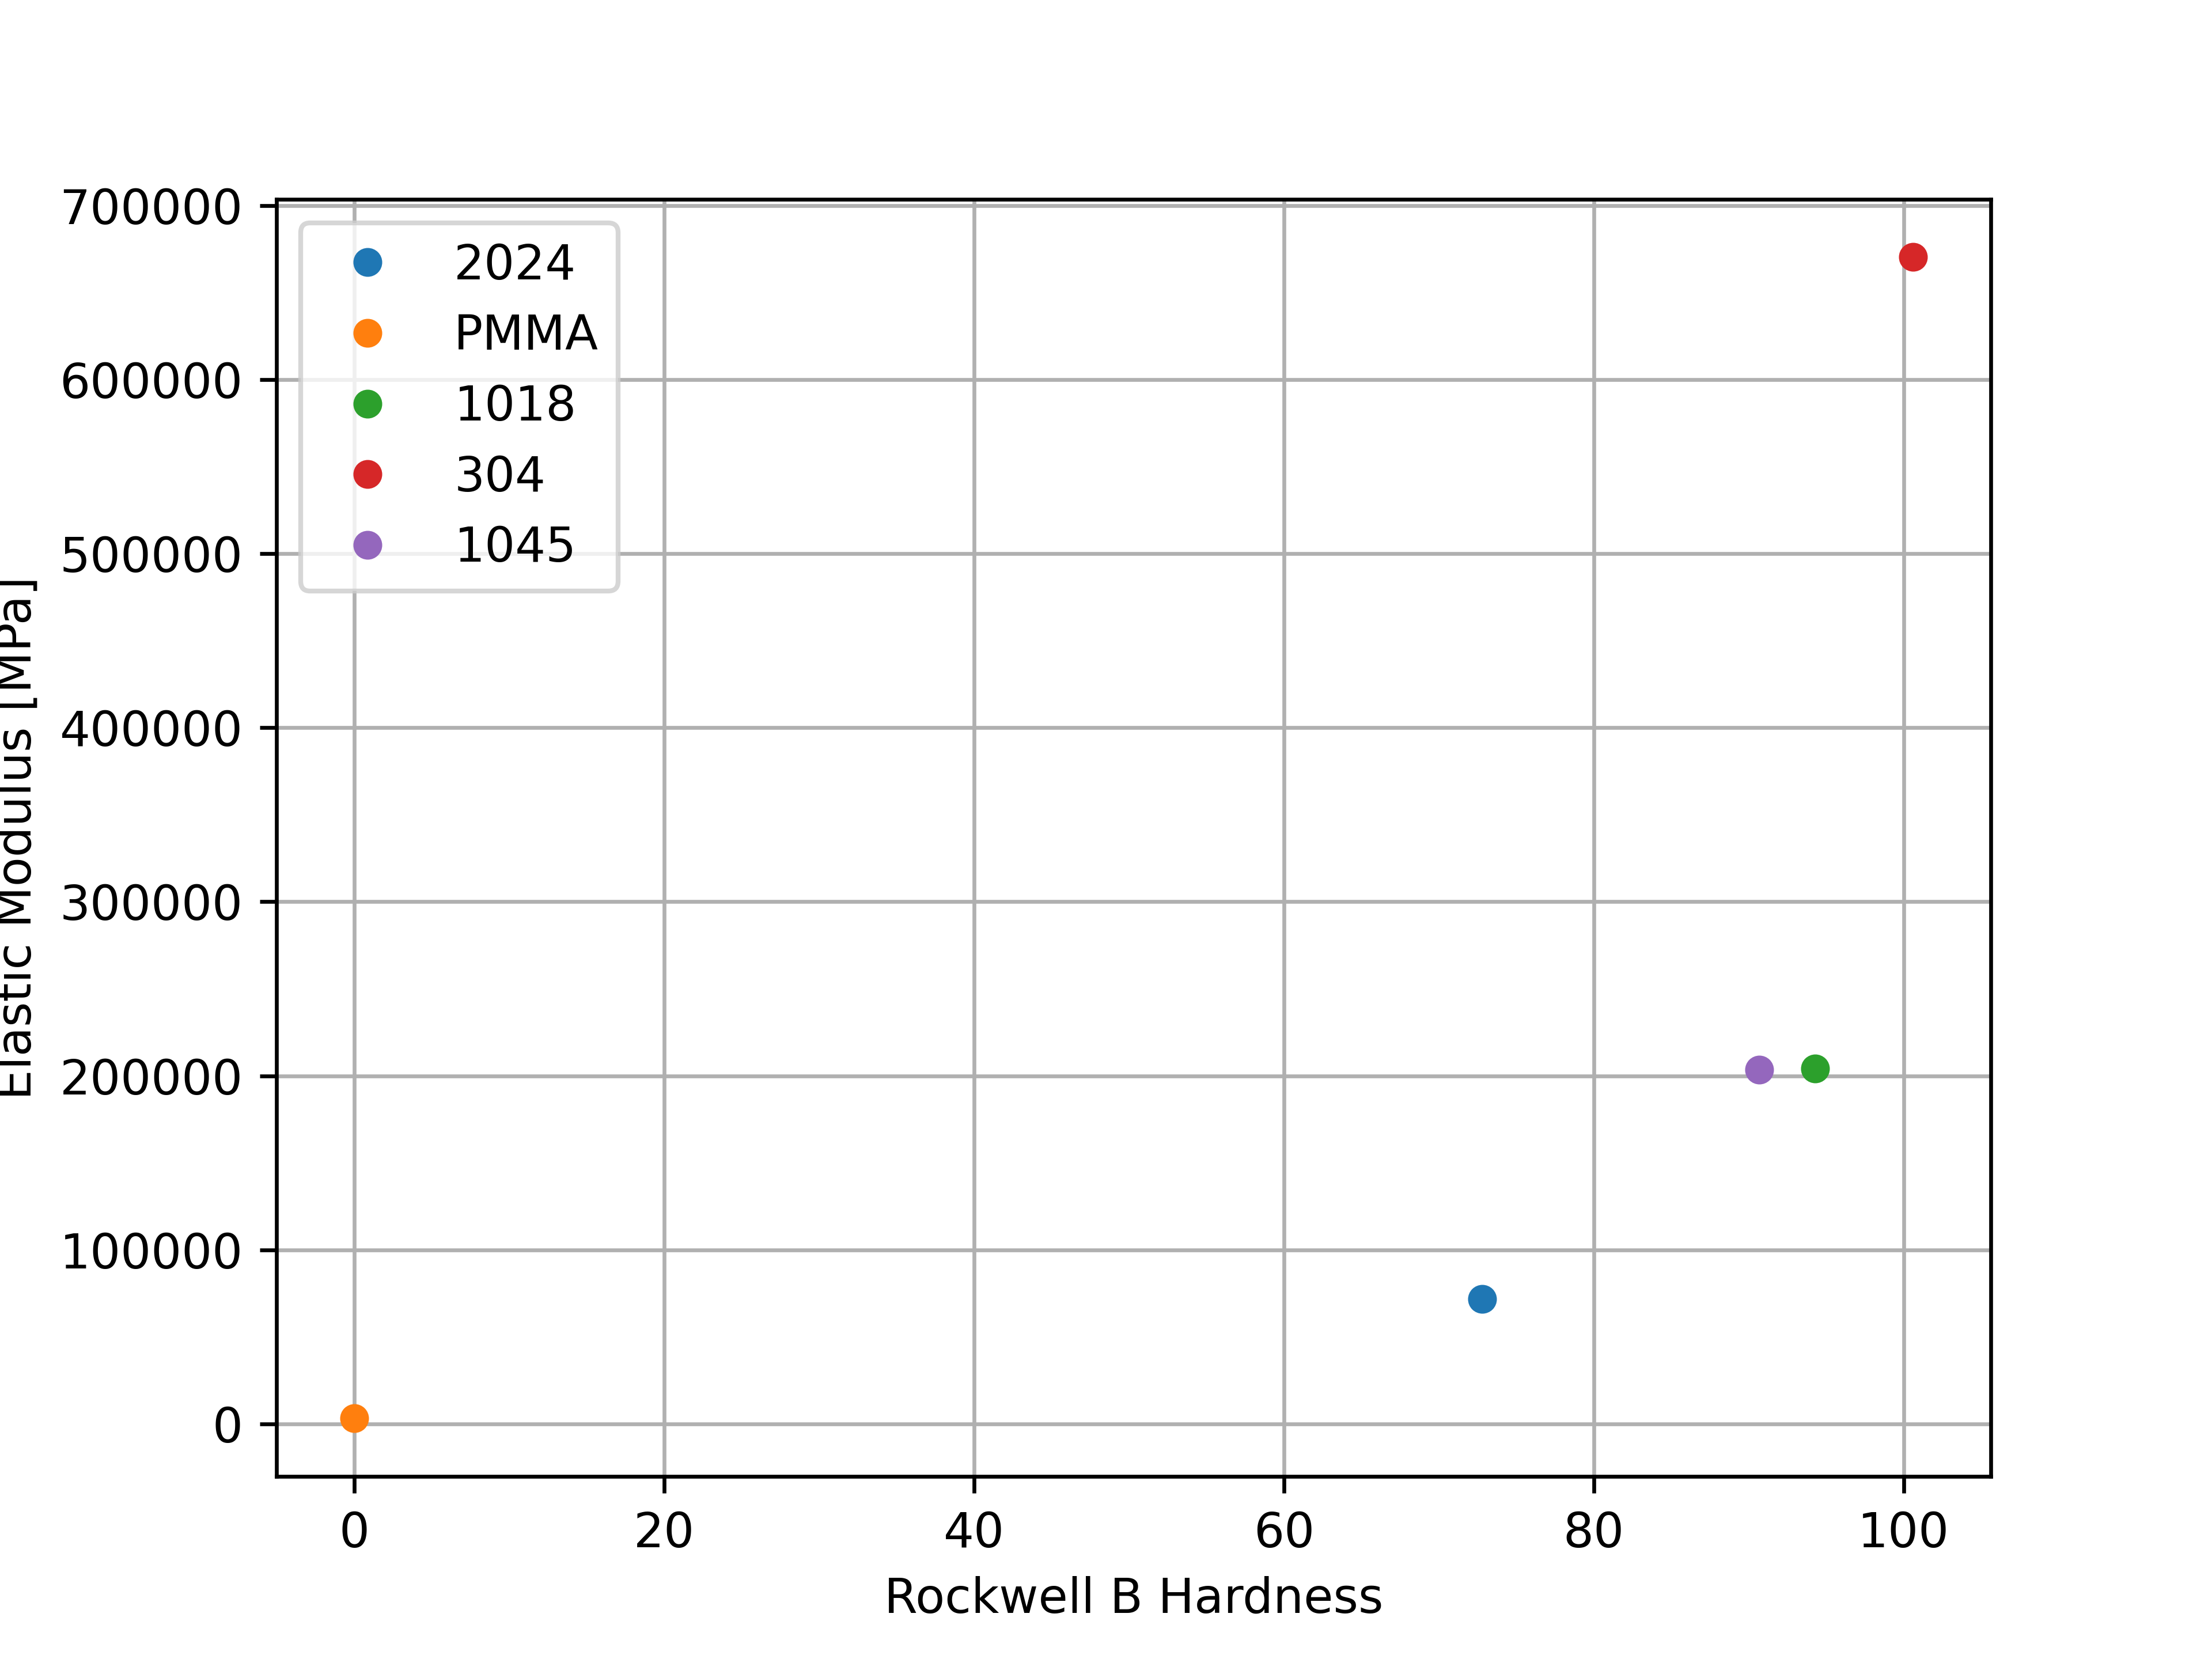
\includegraphics[width=\linewidth]{plots/q3_E.png} 
    \caption{Elastic Modulus as a function \\  of material hardness} 
    \label{figq3:elasmod}
    \vspace{4ex}
  \end{minipage}
  \begin{minipage}[b]{0.5\linewidth}
    \centering
    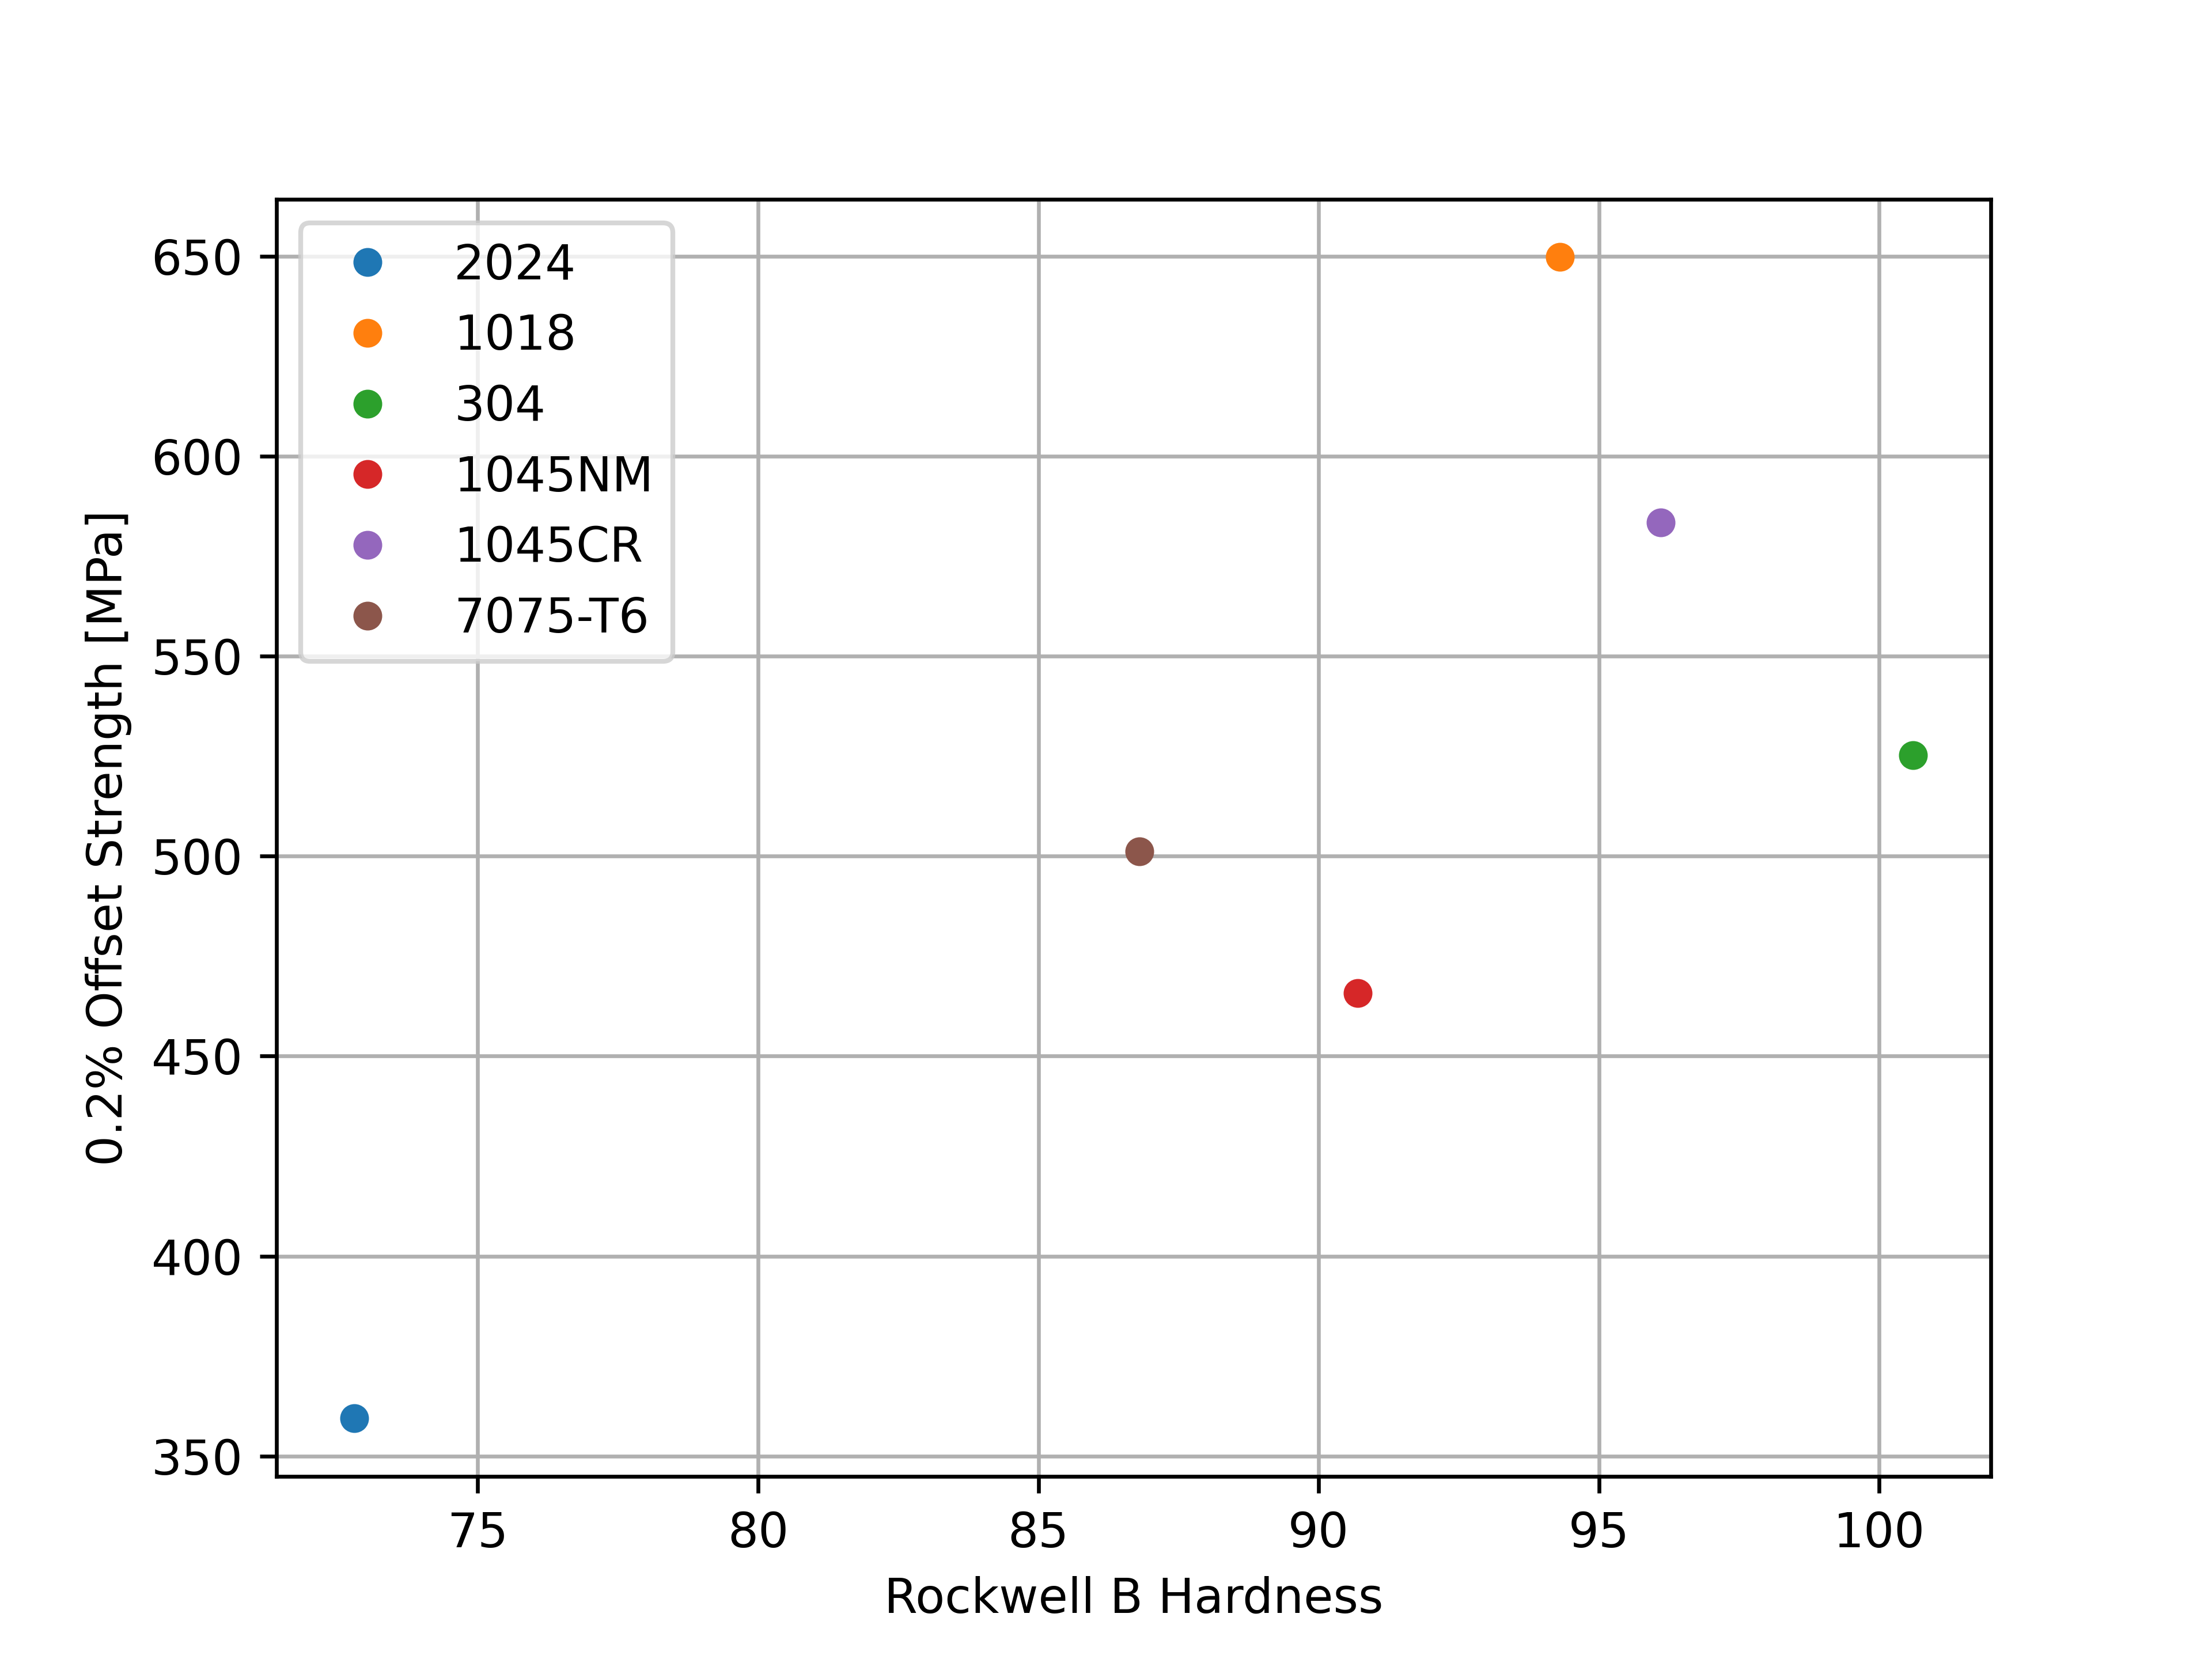
\includegraphics[width=\linewidth]{plots/q3_offstr.png} 
    \caption{Yield Strength as a function \\ of material hardness} 
    \vspace{4ex}
  \end{minipage} 
  \begin{minipage}[b]{0.5\linewidth}
    \centering
    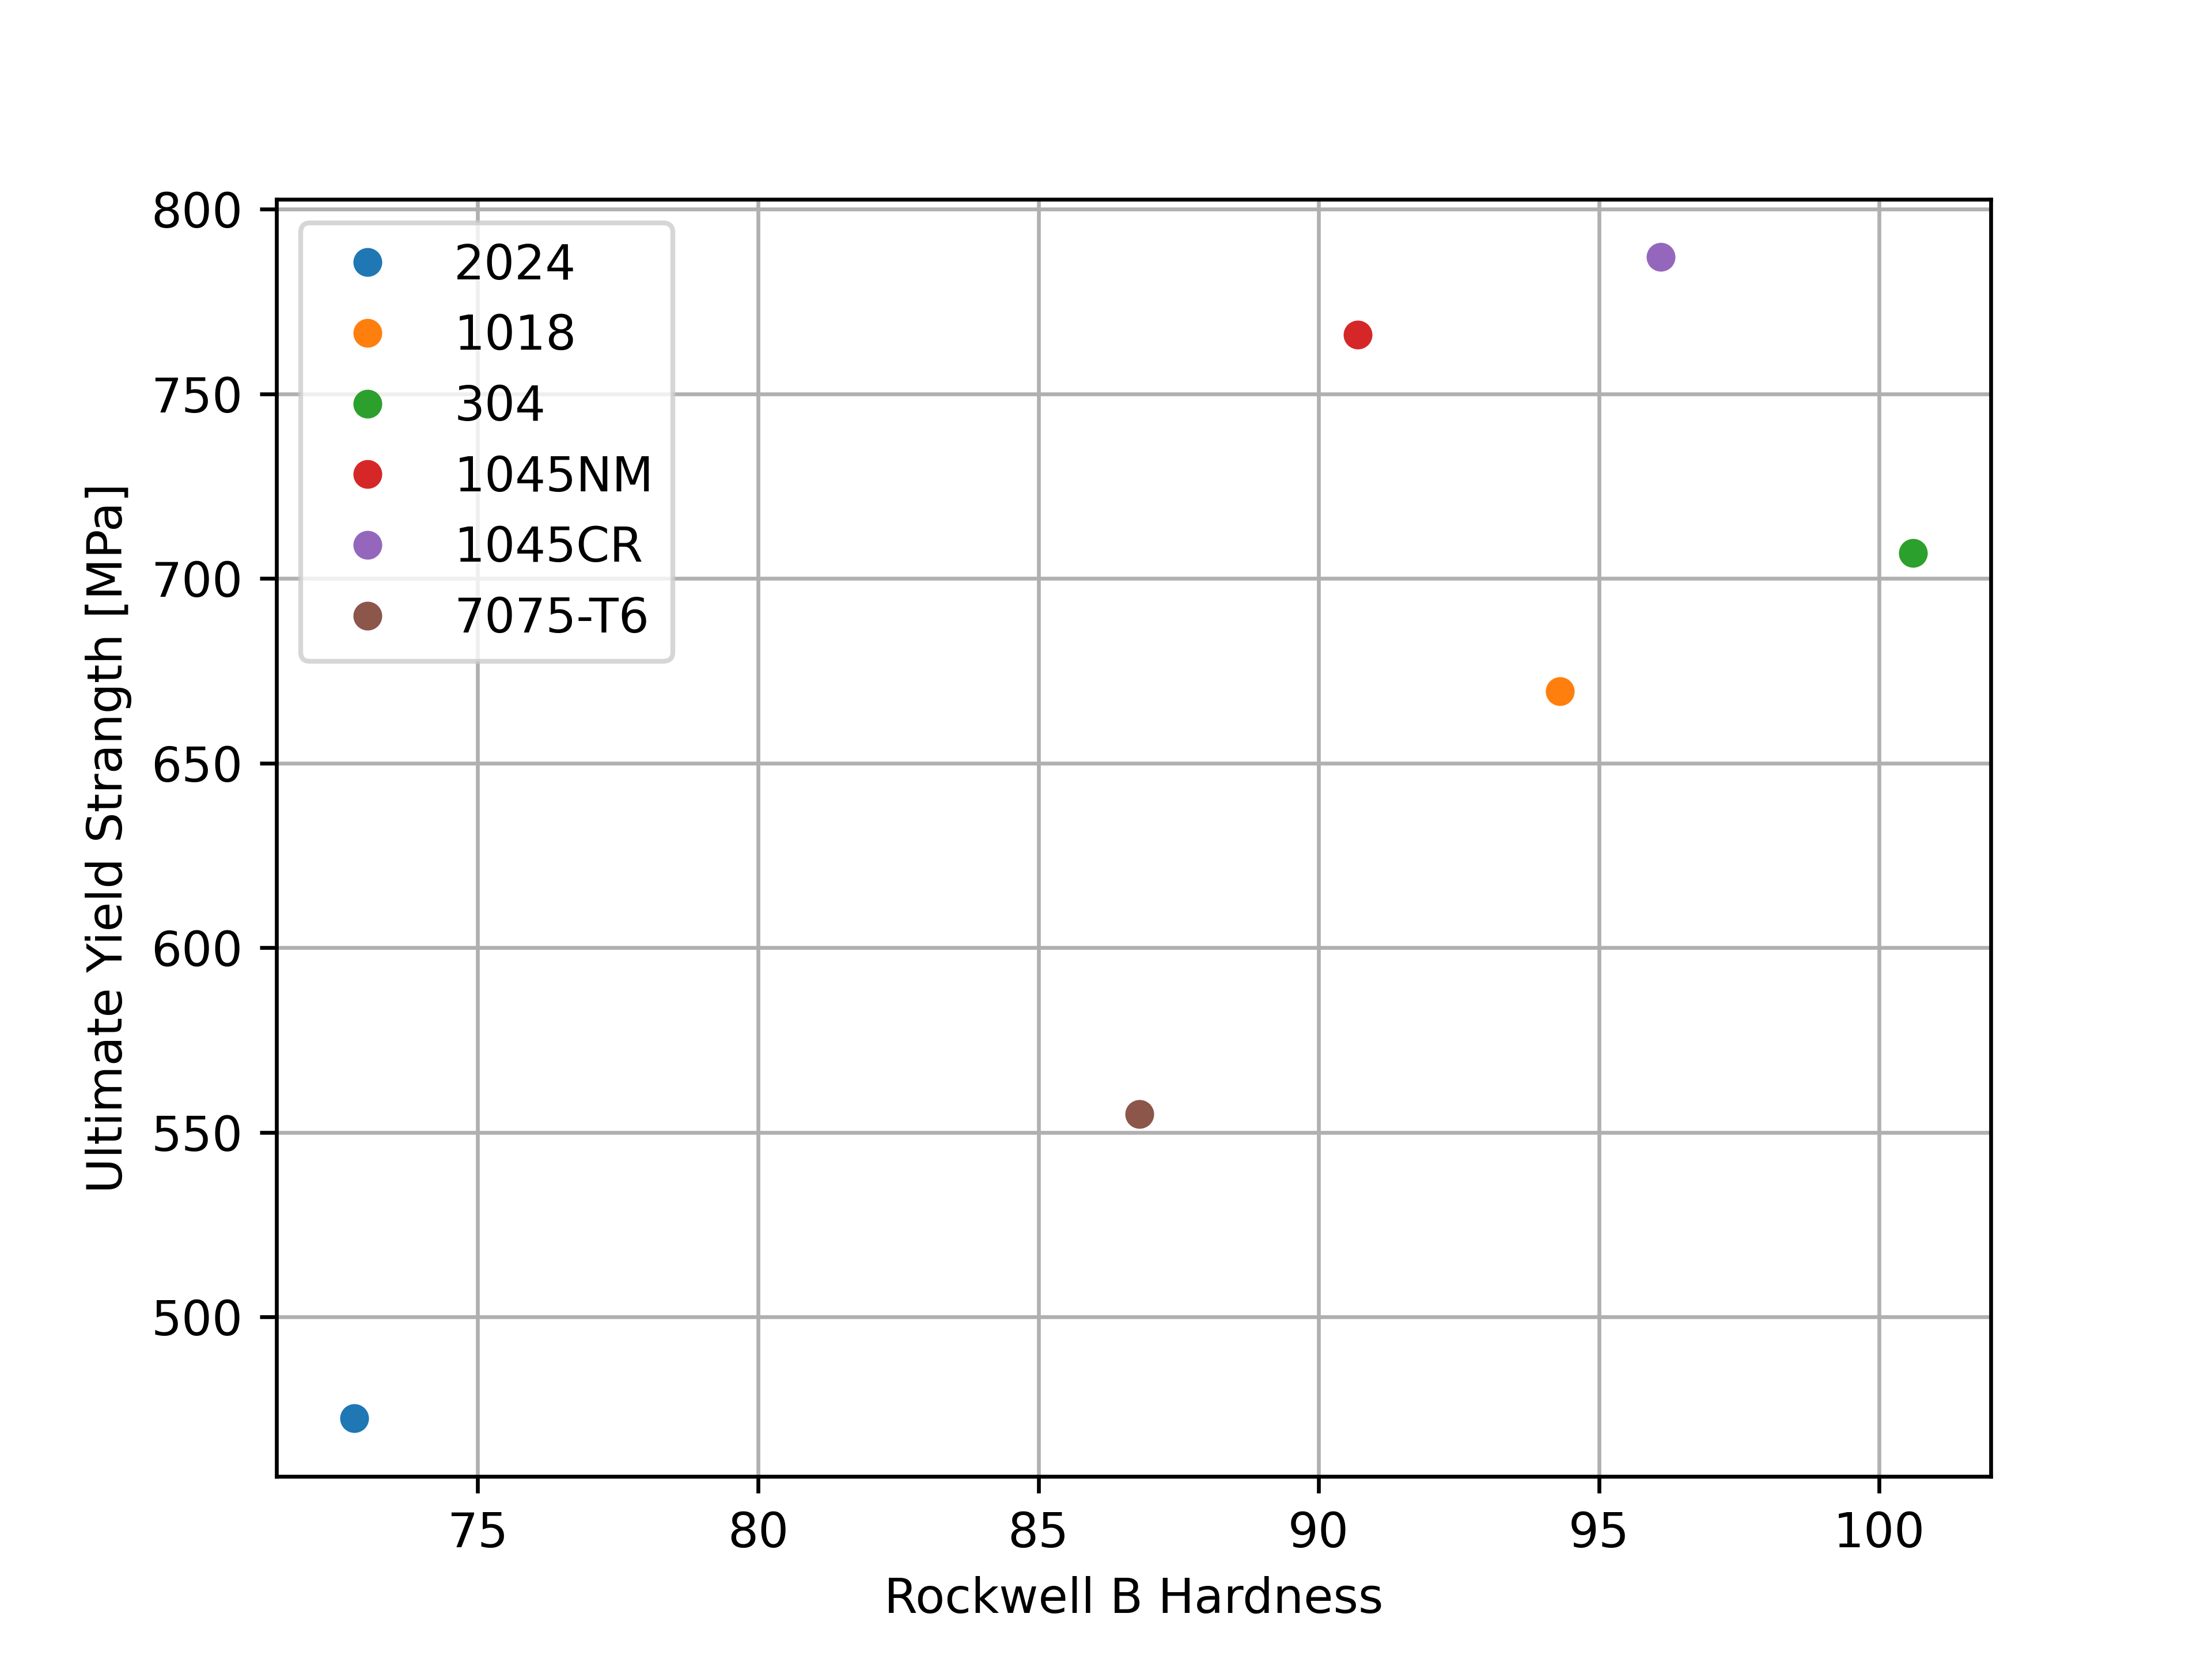
\includegraphics[width=\linewidth]{plots/q3_uts.png} 
    \caption{Ultimate Tensile Strength as a \\ function of material hardness} 
    \vspace{4ex}
  \end{minipage}
  \begin{minipage}[b]{0.5\linewidth}
    \centering
    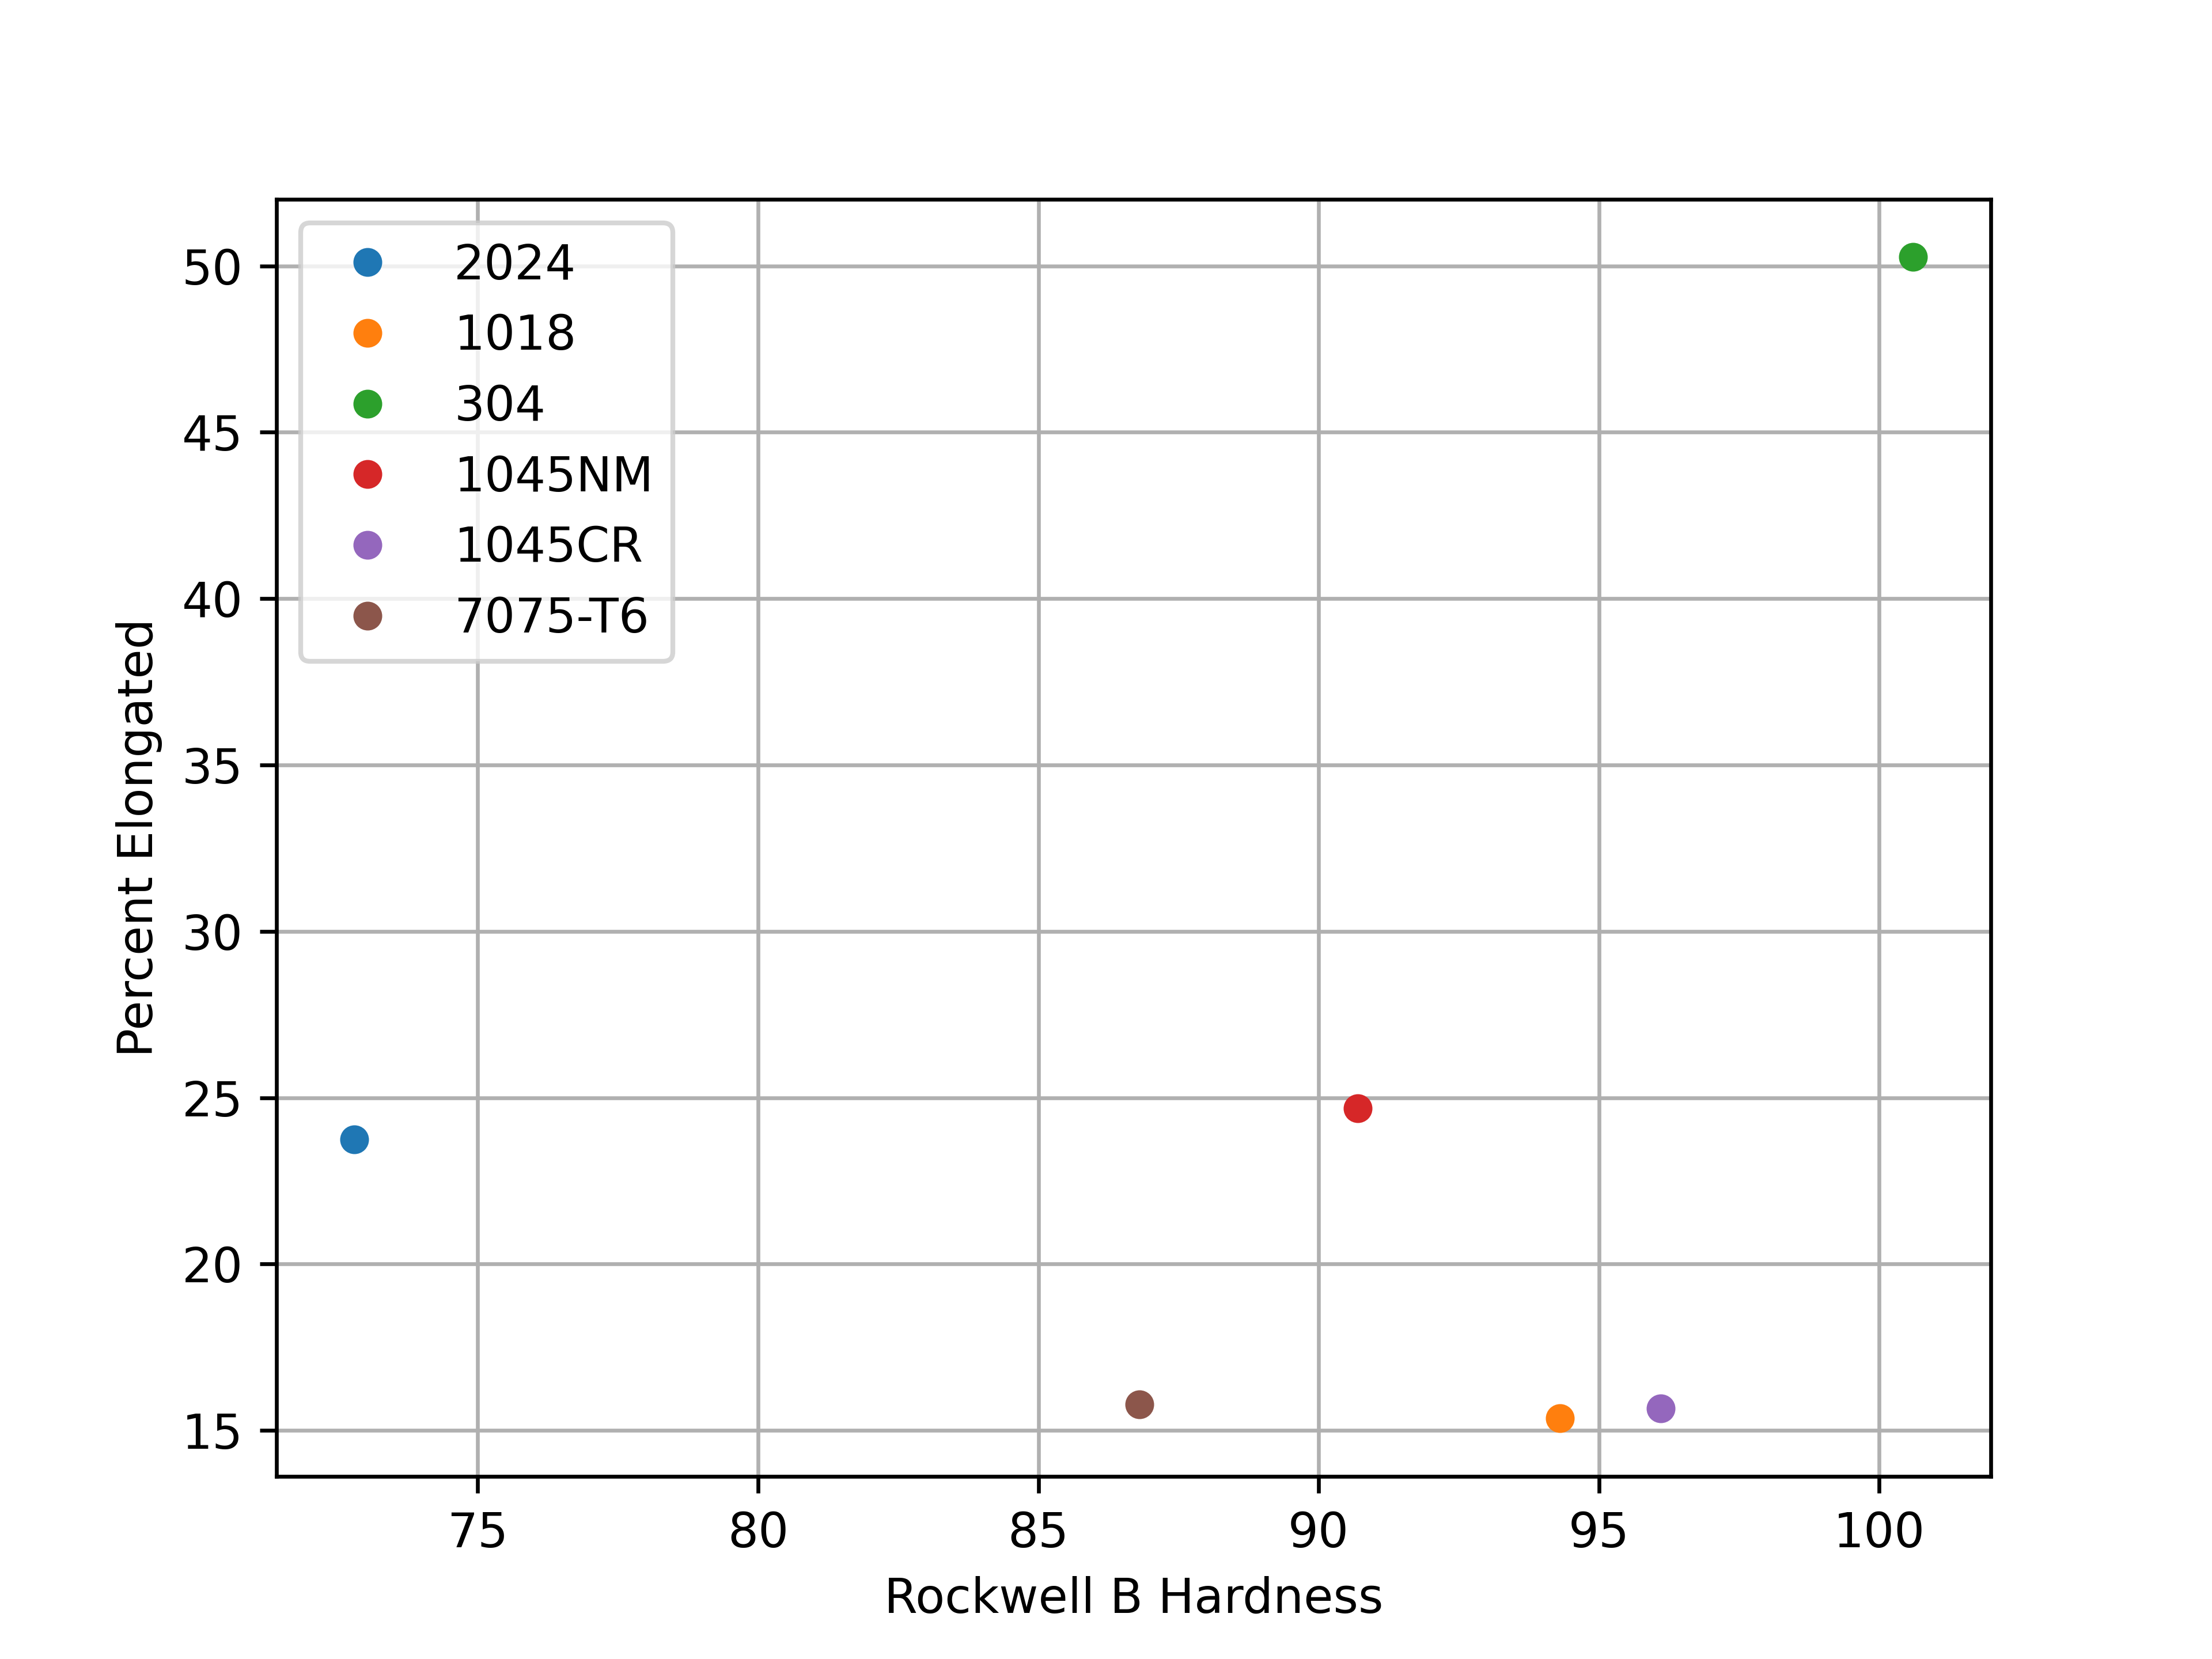
\includegraphics[width=\linewidth]{plots/q3_perelong.png} 
    \caption{Percent Elongation as a function \\ of material hardness} 
    \vspace{4ex}
  \end{minipage} 
  \begin{minipage}[b]{\linewidth}
      \centering
      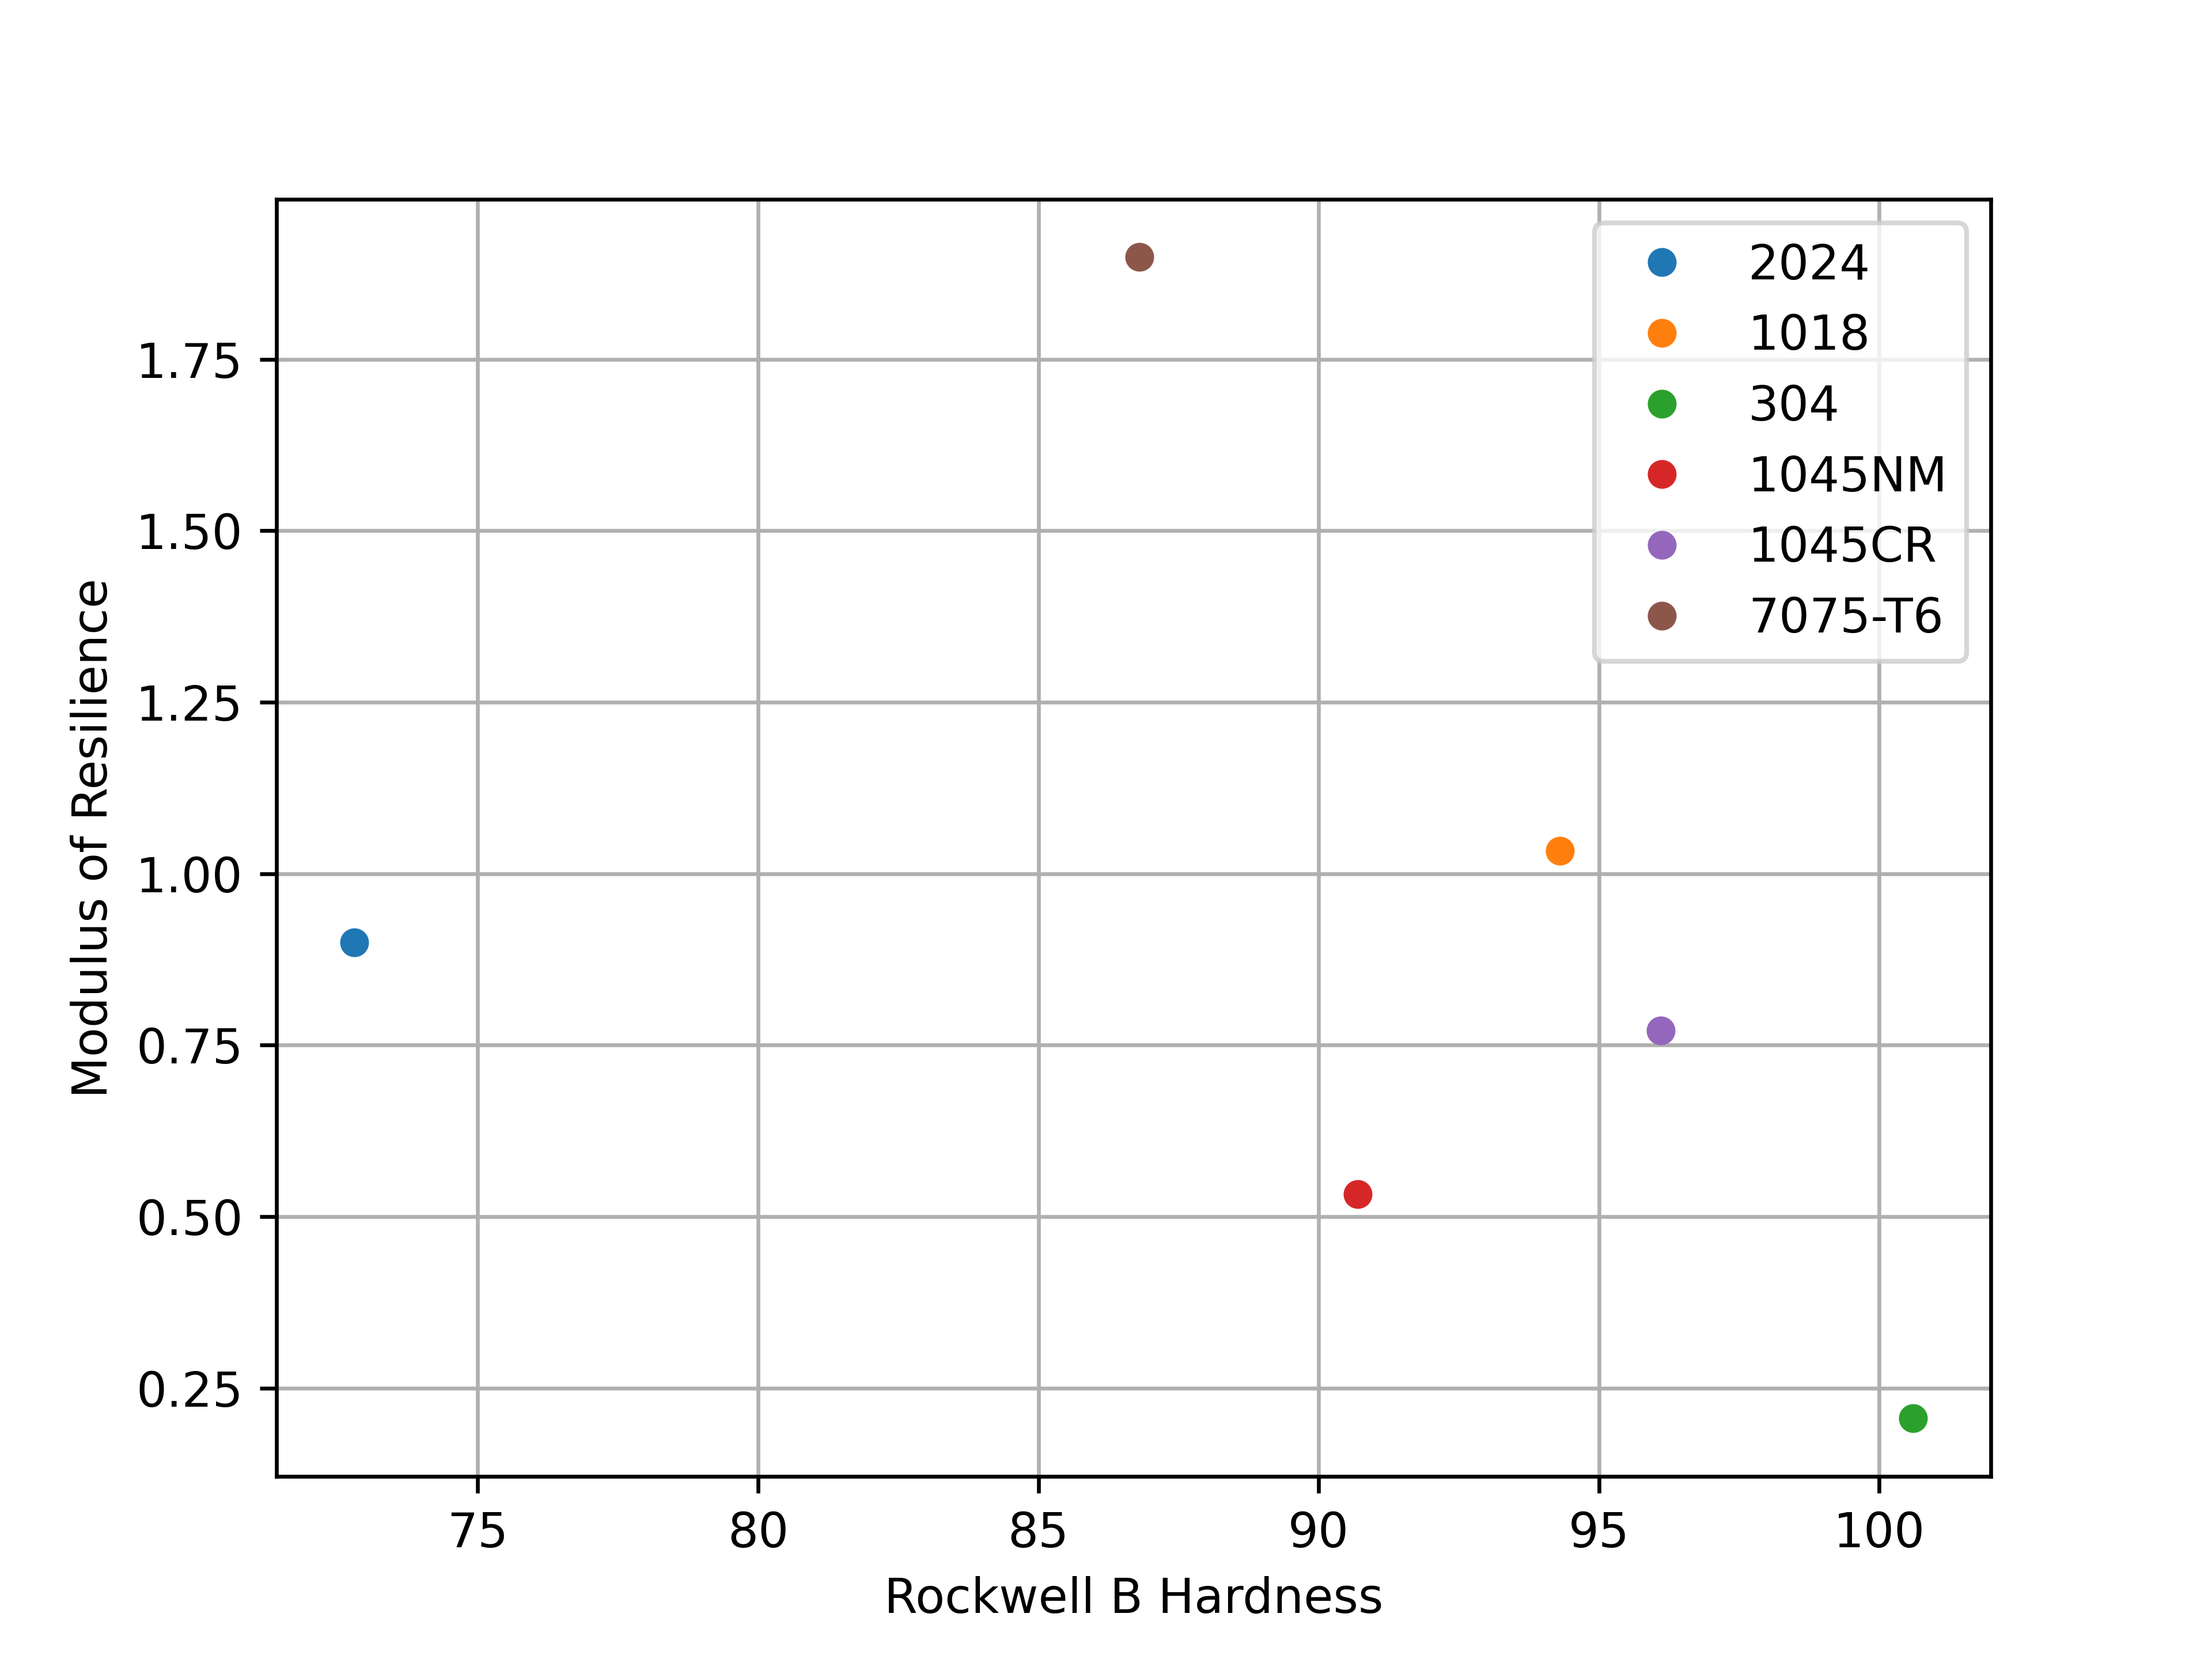
\includegraphics[width = .5\linewidth]{plots/q3_resilmod.png}
      \caption{Modulus of Resilience as a function of material hardness}
      \label{fig:q3resimod}
  \end{minipage}
\end{figure}
\newpage

To continue, for specifically the 304 Stainless Steel, we converted from engineering to true stress/strain utilizing Eqs. \ref{eq:trustress} and \ref{eq:trustrain}. We plotted this in conjunction with the engineering stress/strain curve for the sake of comparison. The resulting figure is presented in Fig. \ref{fig:q4evt}.
\begin{figure}[!h]
    \centering
    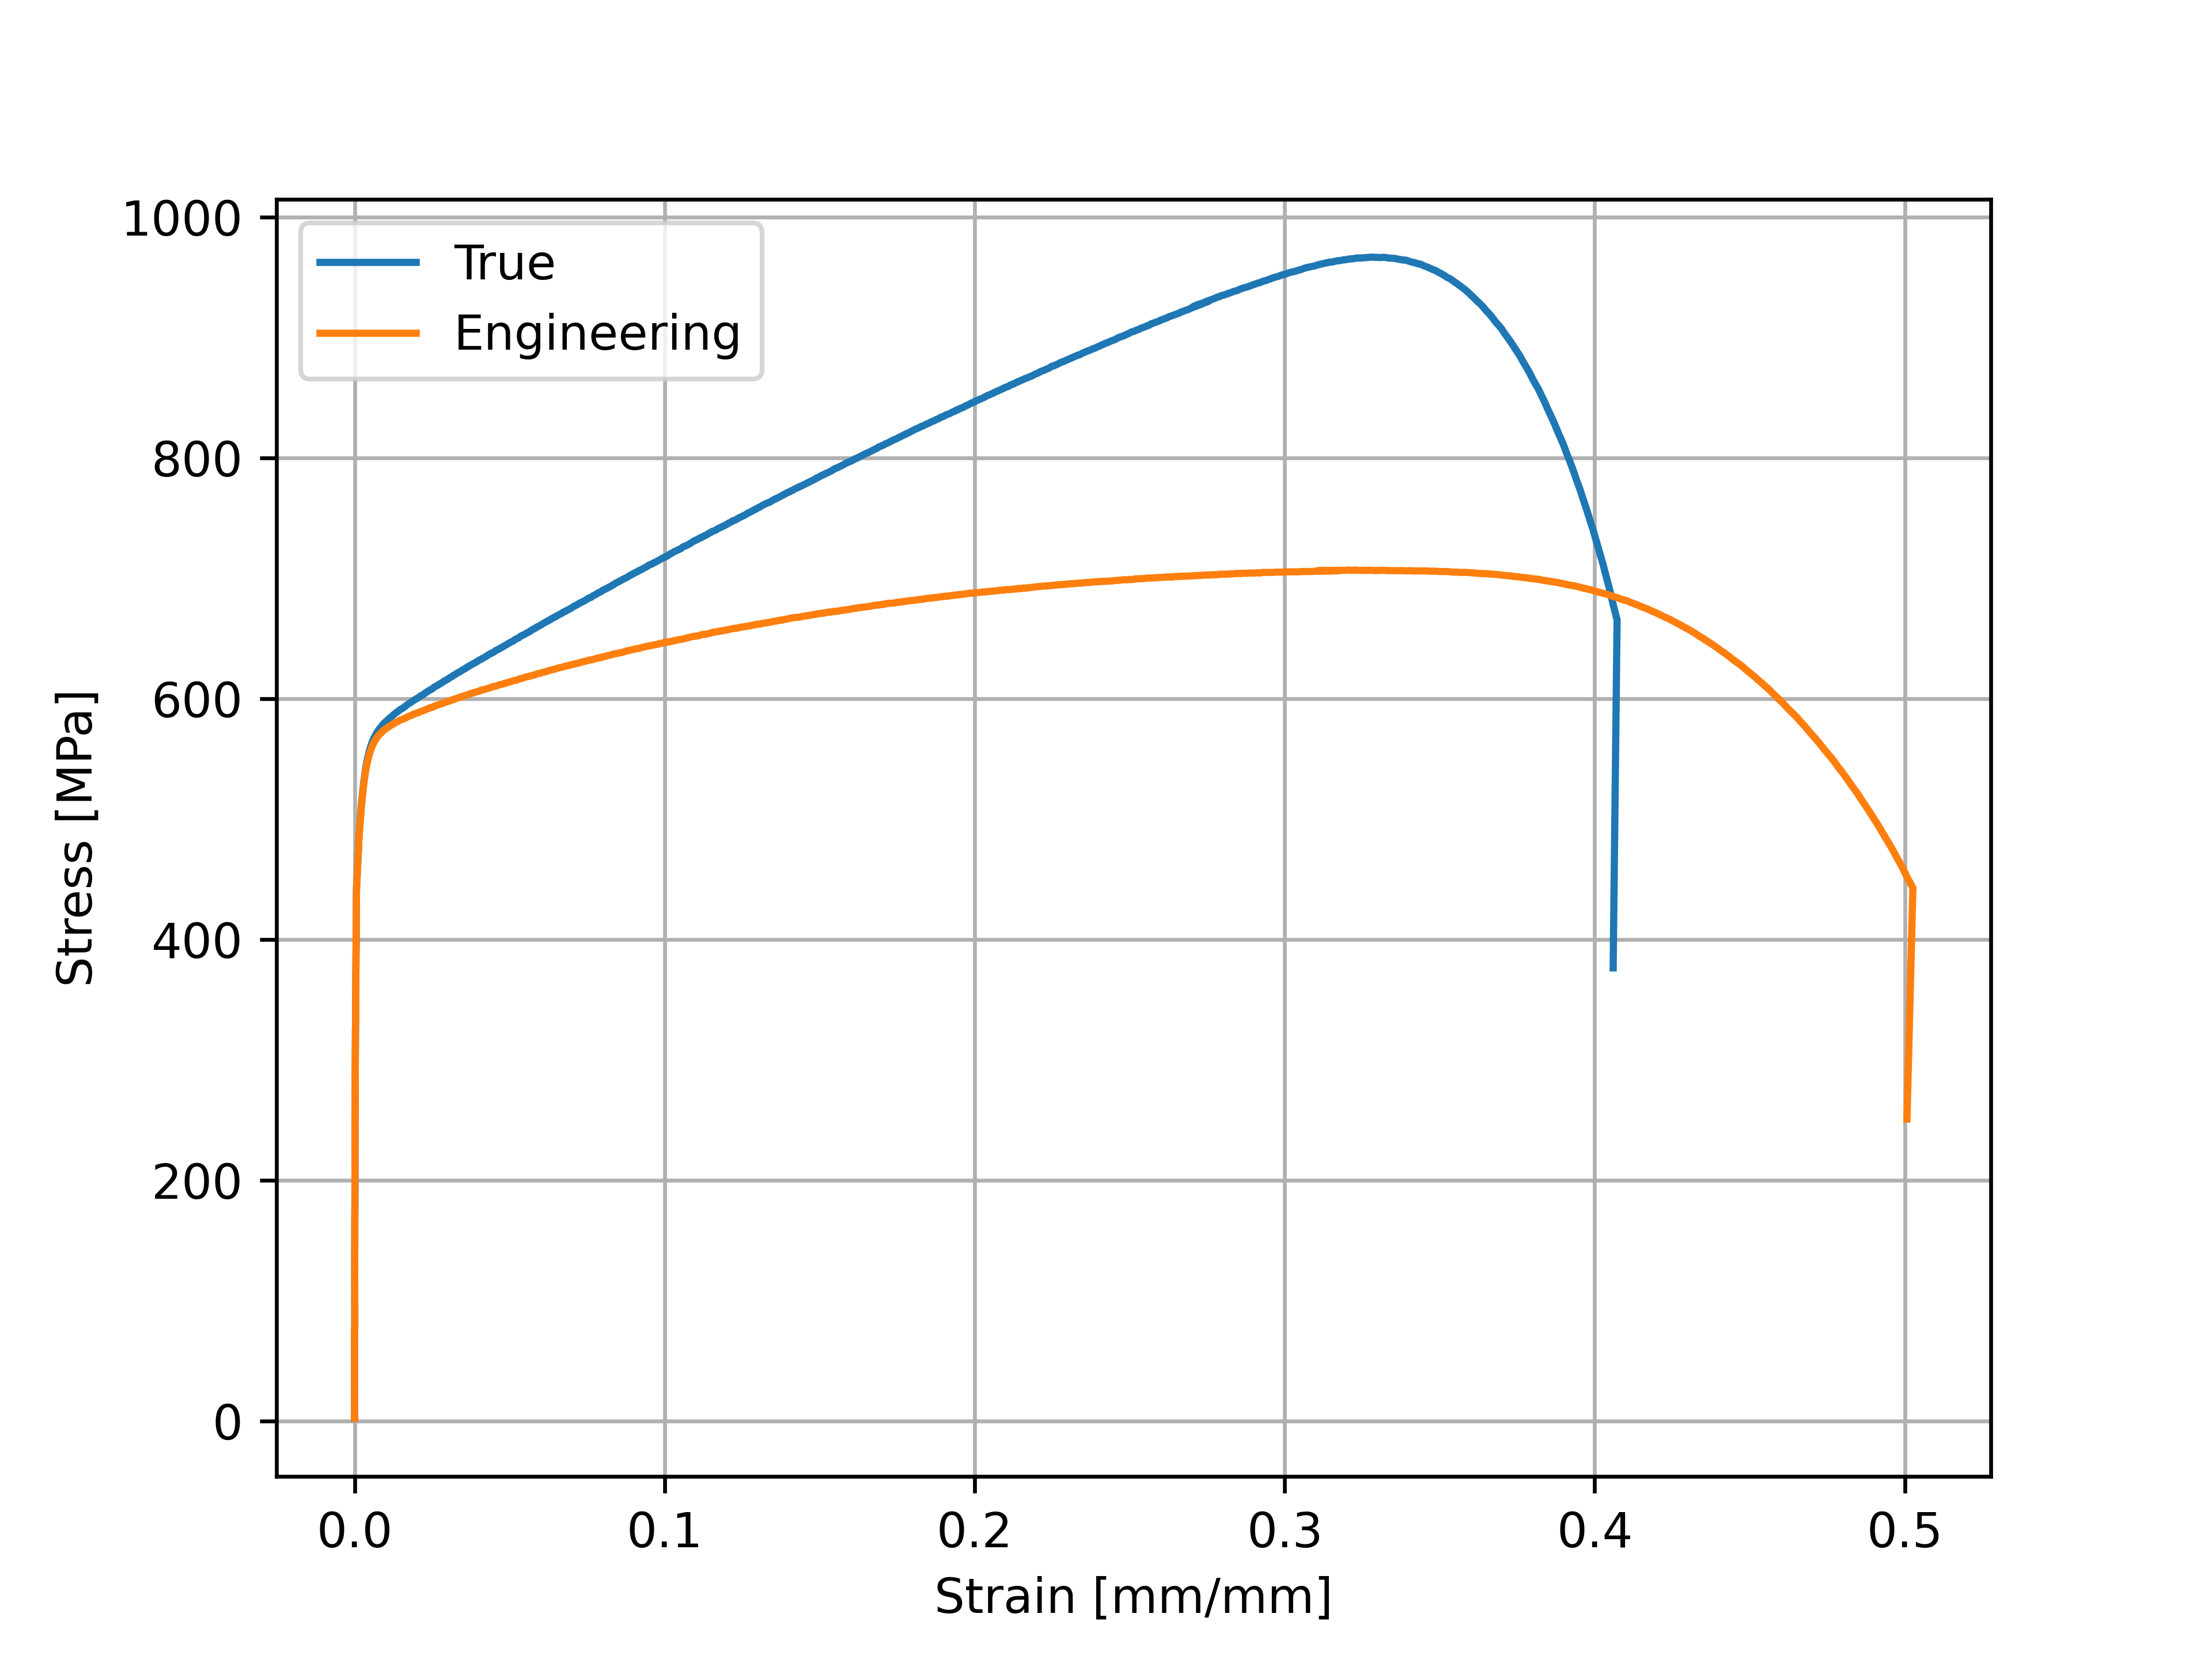
\includegraphics[width=0.5\linewidth]{plots/q4_evt.png}
    \caption{304 Stainless Steel engineering and true stress-strain}
    \label{fig:q4evt}
\end{figure}

From the true stress/strain, we fit the plastic deformation region with a power-law fit, Eq. \ref{eq:powlaw}. To do so, we utilized the \texttt{scipy} python module, specifically \texttt{scipy.optimize.curve\textunderscore fit}. The resulting fit is presented in Fig. \ref{fig:q5fit}. 

\begin{figure}[!h]
    \centering
    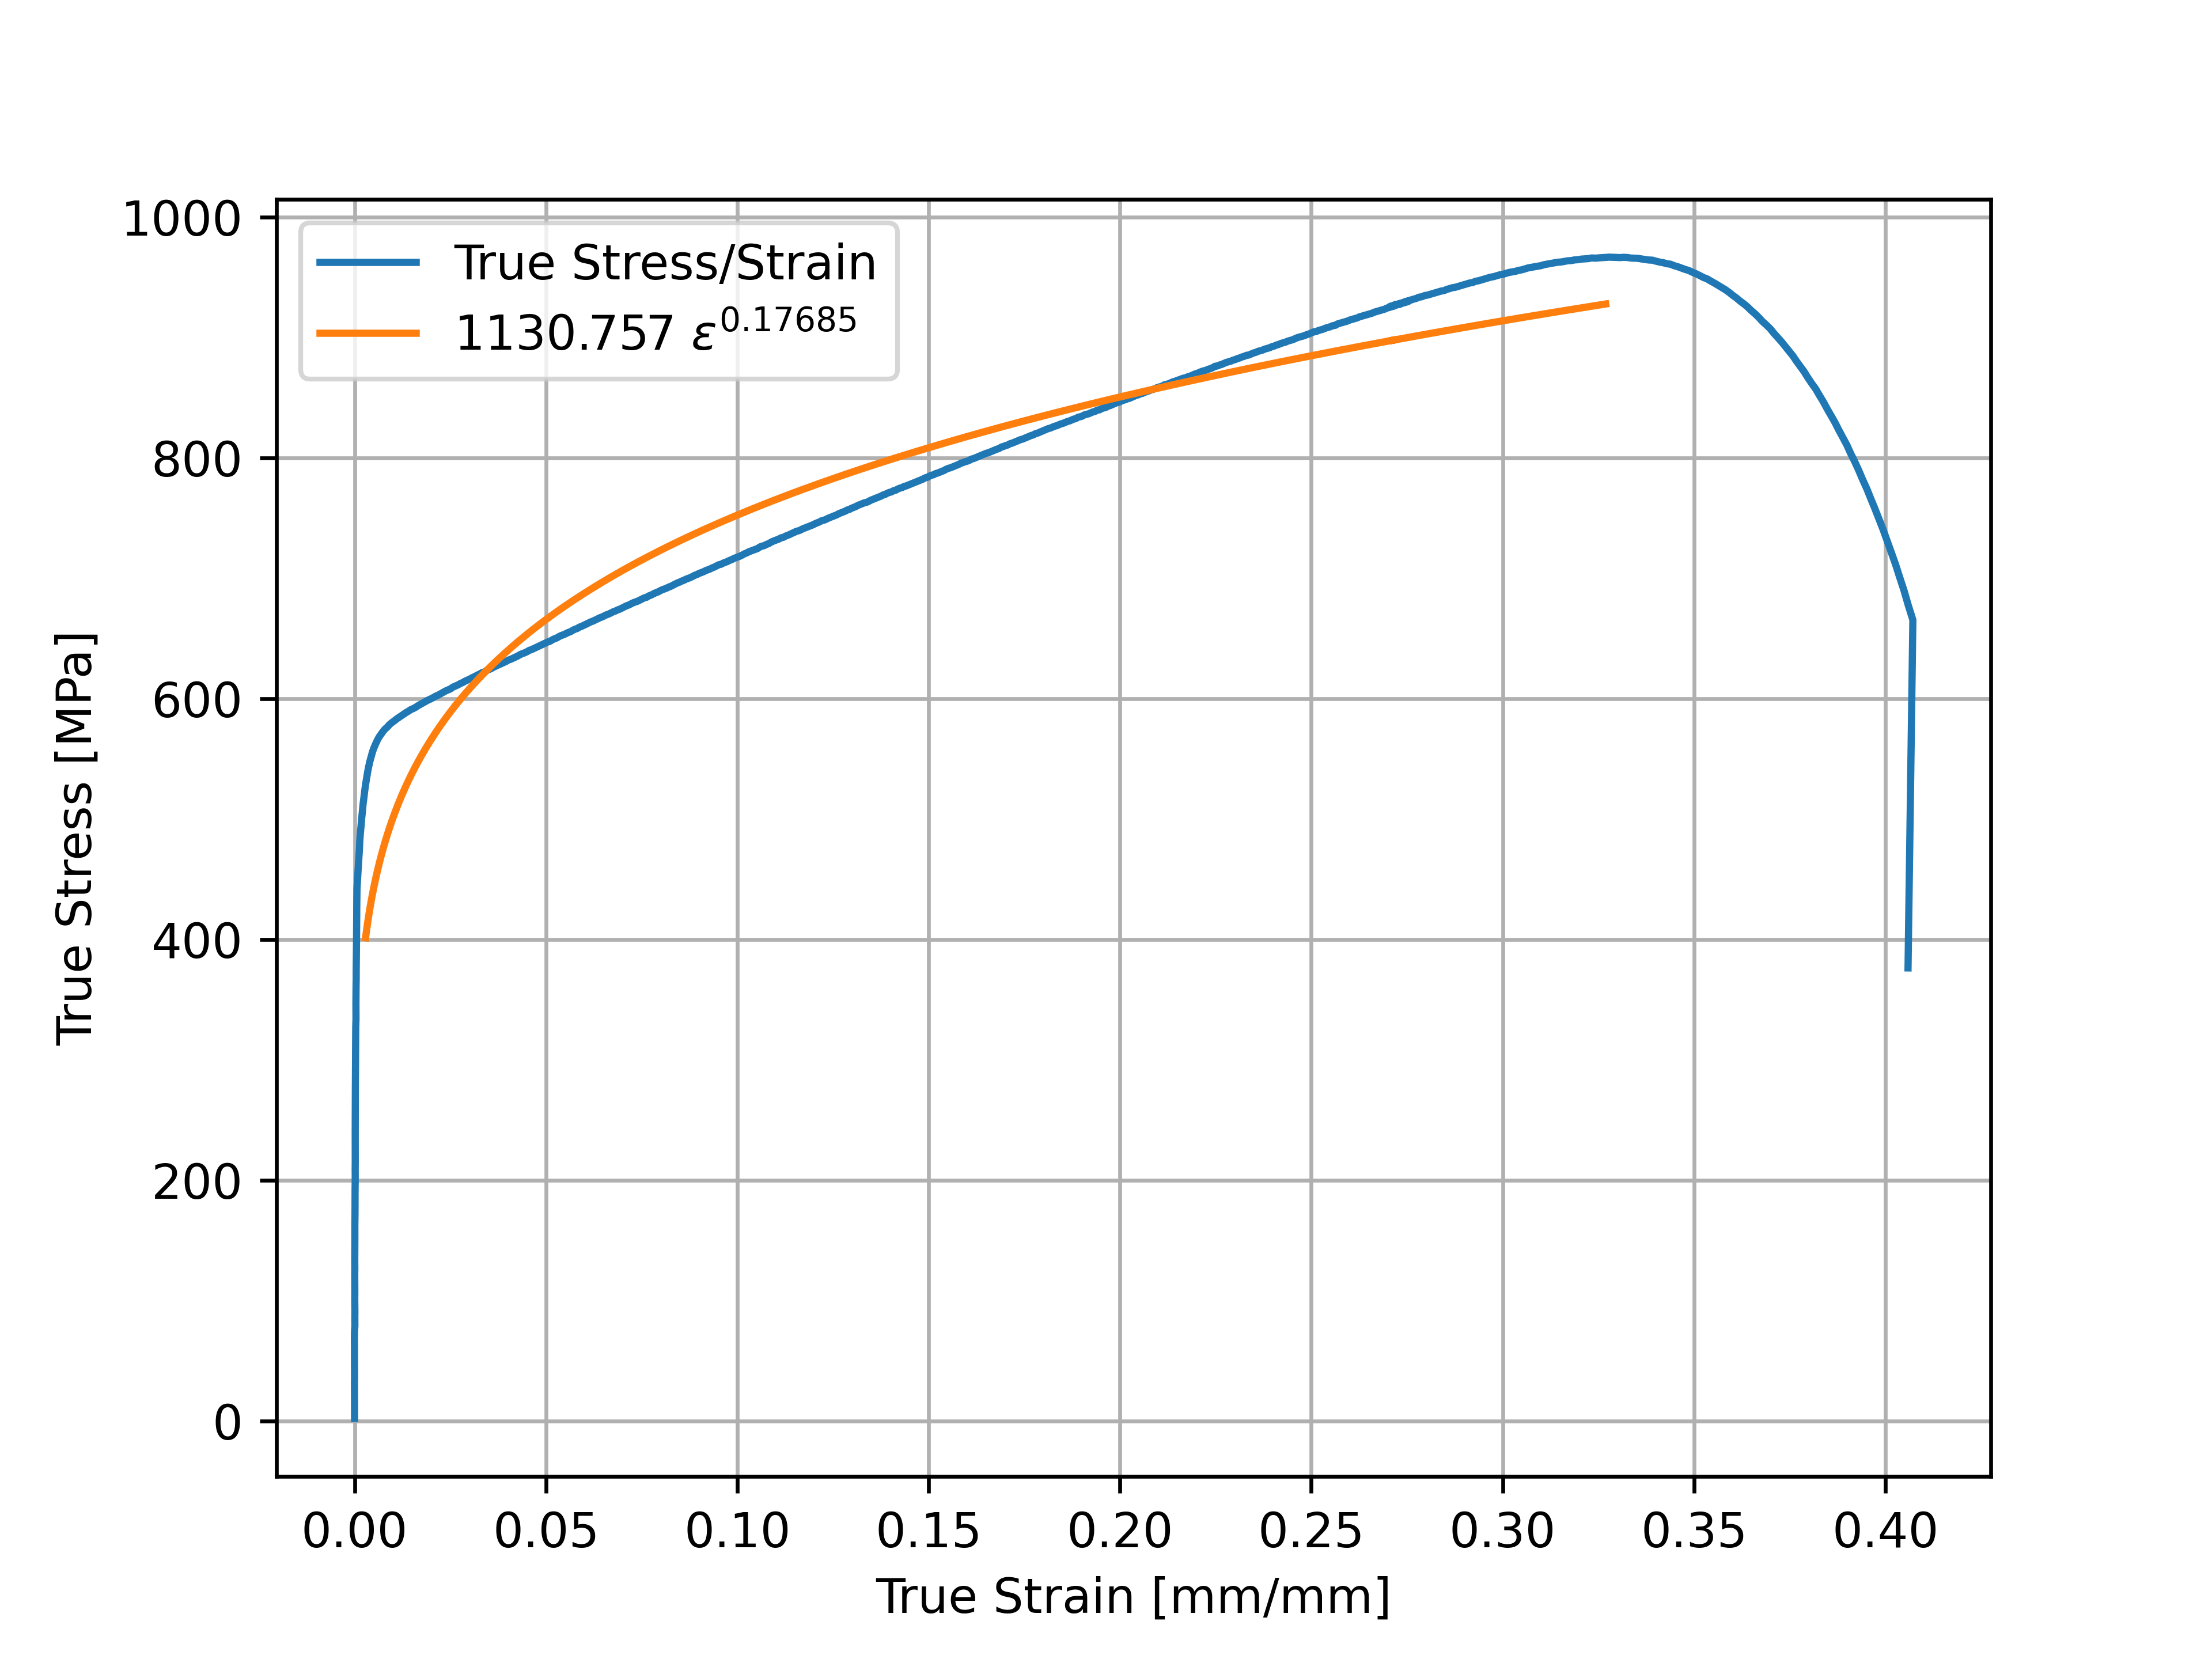
\includegraphics[width=0.5\linewidth]{plots/q5_fit.png}
    \caption{Power-Law fit of plastic deformation of 304 Stainless Steel}
    \label{fig:q5fit}
\end{figure}
\newpage

Finally, we performed a multi-phase loading test on a Bronze specimen. This multi-phase loading test was a tensile test with cyclical 'de-loading' phases. From this test we found the engineering stress vs strain curve, presented in Fig. \ref{fig:br}. From the resulting stress/strain curve we determined the Elastic Modulus and Yield Strength of each Elastic region, as well as the plastic strain at the beginning of each loading phase. To determine the Yield strength, we again utilized the 0.2\% Offset method, for the phases defining the 0.2\% Offset to be 0.2\% more strain than the minimum strain of that phase. These values are tabulated in \ref{tab:q6}.

\begin{figure}[!h]
    \centering
    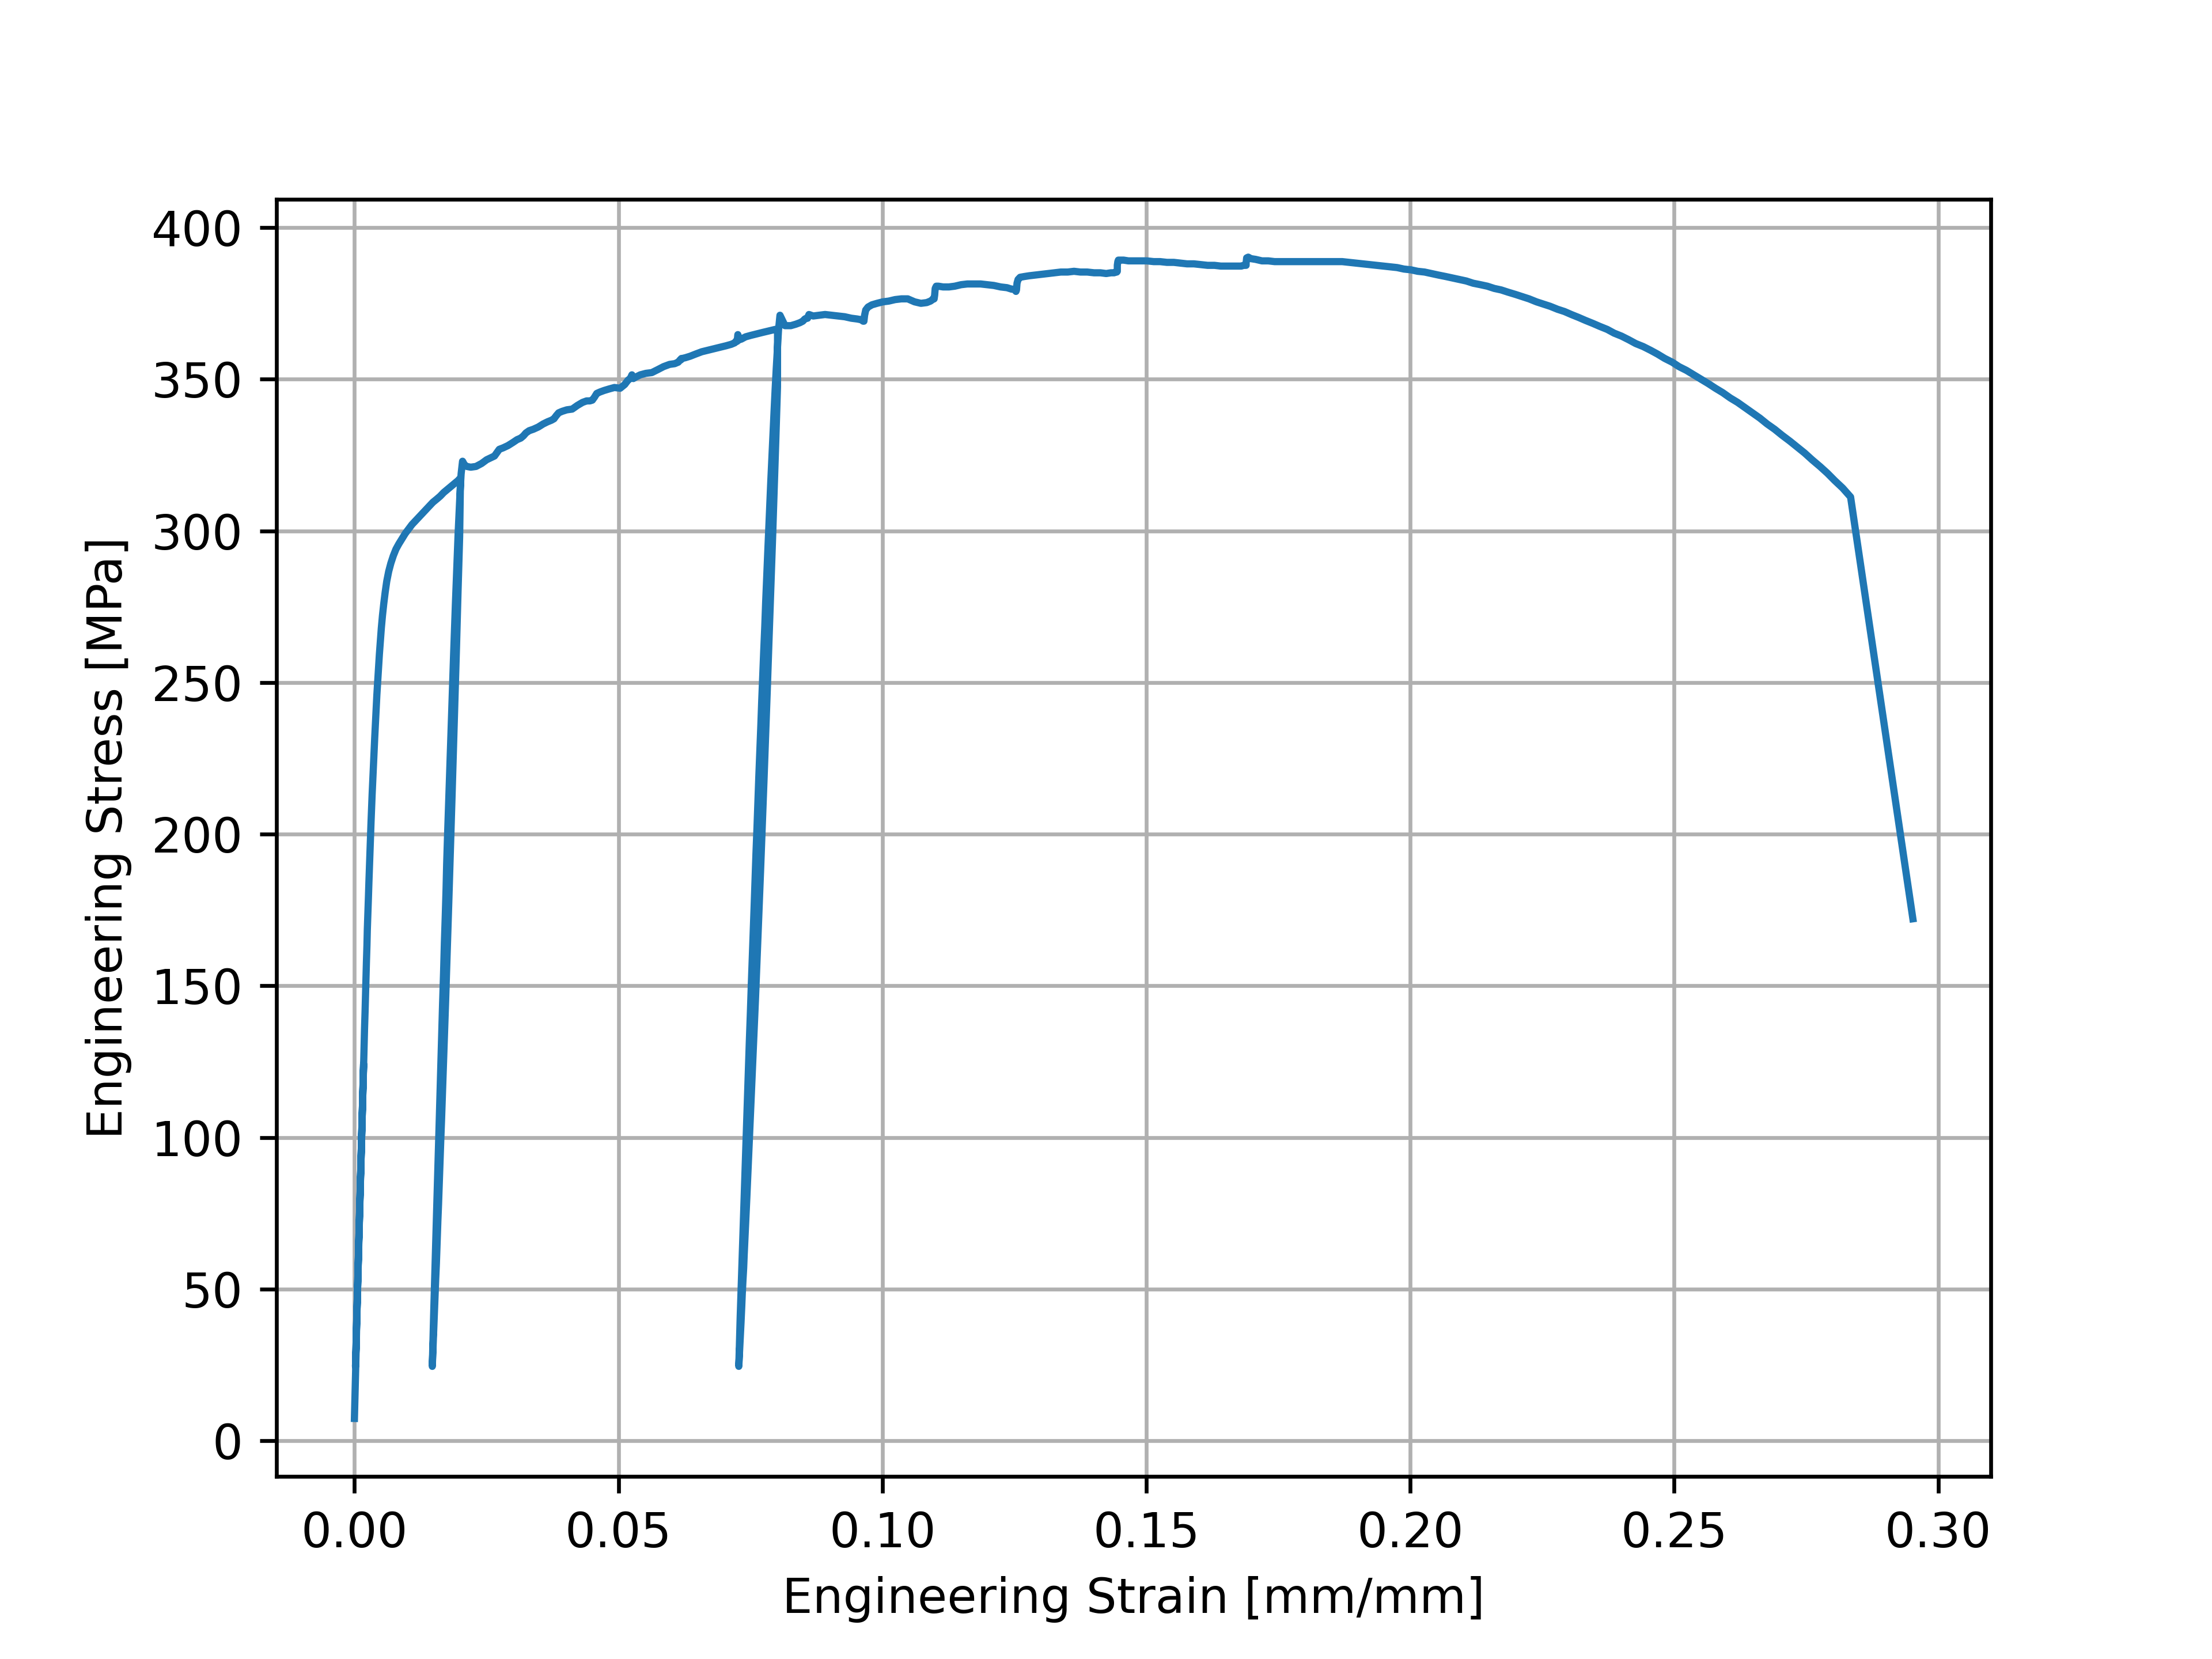
\includegraphics[width=0.5\linewidth]{plots/q6_br.png}
    \caption{Engineering stress-strain of cyclically loaded Bronze}
    \label{fig:br}
\end{figure}

\begin{table}[!h!]
    \centering
    \def\arraystretch{1.5}
    \caption{Material properties at each loading phase of cyclically loaded Bronze}
    \vspace{1pt}
    \begin{tabular}{|c|c|c|c|}
        \toprule
        \hline
        \textbf{Loading Phase} & First & Second & Third \\ 
        \midrule
        \hline
        \textbf{Plastic Strain [\%]} & 0.000 & 1.474 & 7.280 \\
        \textbf{Elastic Modulus [GPa]} & 52.117 & 55.964 & 46.662\\
        \textbf{Yield Strength [MPa]} & 292.9 & 321.1 & 367.7\\

        \hline
    \end{tabular}
    \label{tab:q6}
\end{table}
\newpage

\section{Analysis and Discussion}
\subsection{Analysis of Results}

To begin, in Tab. \ref{tab:q2} the impact of cold rolling (CR) and annealing or normalizing (NM) is apparent, looking specifically at 1045 Steel. CR drastically increases the Yield Strength , the Modulus of Resilience, and the Rockwell B hardness value; whereas NM has much for elongation occur prior to failure. Unsurprisingly, the UTS between the two specimens are nearly identical. Strangely however, the Young's moduli differ by roughly 10\%. This will be discussed further in the final paragraph of this section. To continue, of the select materials in Tab. \ref{tab:q2} each excels in their own right. 304 Stainless Steel is the hardest and by far most ductile; 7075 absorbs the most elastic energy; and cold rolled 1018 Steel is by far the strongest. 

Due to their strong difference in material properties, Steel and Aluminum alloys have wildly different applications. Steel is a strong candidate for structural components, where strength and resistance to deformation are desired and high stress is common; however Aluminum alloys are poor candidates here due to their relative ease to deform under load. On the flip-side, in components were large amounts of strain are expected, Aluminum alloys are a much better candidate due to their ability to resist plastic deformation. 

To continue, the differences between true and engineering stress-strain curves are exemplified in Fig. \ref{fig:q4evt}. Notably, the true stress is much higher than the engineering, whereas the true strain is much lower than engineering. The true stress is much higher than engineering, because as the specimen begins to fail in a tensile test, necking occurs. Necking is where the portion of the specimen being tested is stretching axially and decreasing in cross-sectional area; roughly keeping the volume constant. Because of this decrease in cross sectional area, the force applied to the specimen might be decreasing but the stress is larger because the area bearing the load is decreasing at a faster rate. 

Proximally, the power law fit obtained and presented in Fig. \ref{fig:q5fit} fits the stress/strain curve somewhat well --- this fit has an $R^2$ value of 0.91933. When comparing our values to values in the literature \cite{book}, we notice a strong difference. Accepted values for K and n are 1400 MPa and 0.44, respectively, where our values are 1130.757 and 0.17685, respectively. This difference could be due to the reference material being for annealed 304 Stainless Steel, and we do not know what processes our specimen underwent.

Finally, to discuss the Bronze specimen that underwent cyclical loading. Notably, Young's modulus decreases sharply for the third phase, over a 10\% drop from the first phase. This differs strongly from our in-class theory in which Young's modulus is independent of plastic deformation. This discrepancy is most definitely due to the nature of cold working. Cold working strengthens the material by increases the dislocation density of the material, thus increasing the hardness; but this increase in dislocation density disrupts the elastic movement of the material resulting in a lower Young's modulus at higher plastic deformations. On the contrary, the Yield Strength results are identical to our expected results: as the material goes higher up the stress/strain curve, the strength increases. 

\subsection{Sources of Error}\label{sec:error}
Throughout the experiments, various sources of error had the opportunity to subjugate our results and lead them astray from our theoretical expectations. Prominent sources of error that permeated through all of our experimental trials were scratching from caliper measurements on the gage and improper loading of specimens into the tensile test apparatus. Scratches on the gage portion of the specimen could, during tension, locally increase stress and potentially propagating as a crack throughout the specimen, effectively reducing both the strength and measured percent elongation. Further, improper loading of the specimens could yield unforeseen errors, such as a disagreeing between measured load applied and actual load applied.  

\newpage
\section{Conclusions}
In conclusion, We conducted tension tests on 8 materials to determine various material properties pertaining to strength, elasticity, ductility, and hardness. We investigated Aluminum Alloy 2024, PMMA, Cold Rolled 1018 Steel, 304 Stainless Steel, 1045 Steel (both Cold Rolled and Annealed), and Aluminum Alloy 7075. We determined the elastic moduli, yield strengths, ultimate tensile strengths, percent of elongation, modulus of resilience, and hardness values on the Rockwell B scale. We investigated the change of these values as a function of material hardness. Further, we investigated the differences between true and engineering stress/strain, and the applicability of a power-law fit to the plastic deformation region of the true stress/strain curve of 304 Stainless Steel. Lastly, we investigated the effects of plastic deformation on the elastic modulus and yield strength of Bronze. We found that material properties pertaining to strength, elasticity, and ductility vary strongly with hardness. We found true stress is larger than engineering, and true strain is smaller than engineering, and that a power-law fit is well adept to approximating the plastic deformation region of the stress/strain curve for 304 Stainless Steel. Finally, we found that as plastic deformation increases so does the yield strength of the material, conversely the elastic modulus decreases slightly. 

\section{References}
\printbibliography[heading=none]

\end{document}